\documentclass[11pt, a4paper]{report}

% ----- PACKAGES -----
\usepackage[utf8]{inputenc}
\usepackage{amsmath}
\usepackage{amssymb}
\usepackage{amsfonts}
\usepackage{graphicx}
\usepackage[margin=0.8in]{geometry}
\usepackage{hyperref}
\usepackage{svg}
\usepackage{fancyhdr}
\usepackage{titlesec}
\usepackage{wrapfig}
\usepackage{xcolor}
\usepackage{subcaption}
\usepackage{float}


\hypersetup{
    colorlinks = true,
    linkcolor  = blue,
    filecolor  = magenta,
    urlcolor   = cyan
}


% Optional: make links blue but not boxed
\hypersetup{
    colorlinks=true,
    linkcolor=blue,
    urlcolor=blue,
    citecolor=blue
}
% ----- CHAPTER TITLE CUSTOMIZATION -----
\titleformat{\chapter}[display]
  {\normalfont\Large\bfseries}
  {\chaptertitlename\ \thechapter}
  {1em}
  {}
\titlespacing*{\chapter}
  {0pt}
  {5pt}
  {15pt}

\titleformat{\section}
  {\normalfont\Large\bfseries\itshape} % bold + italic for section titles
  {\thesection}{1em}{}

\titleformat{\subsection}
  {\normalfont\large\bfseries\itshape} % italic, same size as default subsection
  {\thesubsection}{1em}{}

\titleformat{\subsubsection}
  {\normalfont\normalsize\bfseries\itshape} % italic, same size as default subsubsection
  {\thesubsubsection}{1em}{}

% ----- HEADER & FOOTER SETUP -----
\pagestyle{fancy}
\fancyhf{}
\fancyhead[L]{\nouppercase{\leftmark}}
\fancyfoot[C]{\thepage}
\renewcommand{\headrulewidth}{1pt}
\renewcommand{\footrulewidth}{1pt}

% ----- TITLE PAGE INFORMATION -----
\title{Notes: Special Relativity and Flat Spacetime}
\author{Abdelrahman Mohamed Anwar}
\date{\today}

% add: clickable equation reference macro (uses hyperref)
\newcommand{\eqn}[1]{\hyperref[#1]{\eqref{#1}}}

%%%%%%%%%%%%%%%%%%%%%%%%%%%%%%%%%%%%%%%%%%%%%%%%%%%%%%%%%%%%%%%%%%%%%%
% DOCUMENT BEGINS
%%%%%%%%%%%%%%%%%%%%%%%%%%%%%%%%%%%%%%%%%%%%%%%%%%%%%%%%%%%%%%%%%%%%%%
\begin{document}

\maketitle
\thispagestyle{empty}
\newpage

\tableofcontents
\newpage

%%%%%%%%%%%%%%%%%%%%%%%%%%%%%%%%%%%%%%%%%%%%%%%%%%%%%%%%%%%%%%%%%%%%%%
% MAIN CONTENT
%%%%%%%%%%%%%%%%%%%%%%%%%%%%%%%%%%%%%%%%%%%%%%%%%%%%%%%%%%%%%%%%%%%%%%
\chapter{Manifolds}

\section{Gravity as Geometry}

The foundational insight of general relativity is that gravity is not a force that propagates \emph{through} spacetime, but is instead a manifestation of spacetime's own geometry. The physical concept that leads to this radical conclusion is the \textbf{Principle of Equivalence}, which formalizes the observed universality of the gravitational interaction. This principle can be formulated in several distinct, progressively stronger ways.

\subsection*{The Weak Equivalence Principle (WEP)}
The WEP states that the \textbf{inertial mass} ($m_i$) and \textbf{gravitational mass} ($m_g$) of any object are equal.

\begin{itemize}
    \item \textbf{Inertial Mass} relates an applied force to the resultant acceleration via Newton's Second Law:
    \begin{equation}
        F = m_i a
    \end{equation}
    \item \textbf{Gravitational Mass} acts as the "gravitational charge," determining the force experienced by an object in a gravitational potential $\Phi$:
    \begin{equation}
        F_g = -m_g \nabla \Phi
    \end{equation}
\end{itemize}

The WEP sets $m_i = m_g$. The immediate and profound consequence is that the acceleration of any test particle in a gravitational field is \emph{independent} of its own mass or composition:
\begin{equation}
    a = -\nabla \Phi
\end{equation}
This universality is unique to gravity. In contrast, in an electric field, particles with different charge-to-mass ratios follow different trajectories.

\subsubsection*{The "Sealed Box" Analogy}
An alternative formulation of the WEP is that an observer in a small, sealed box, by observing the motion of freely-falling particles, cannot distinguish between being in a uniform gravitational field and being in a uniformly accelerating reference frame.

This equivalence is necessarily \emph{local}. In a large enough box, an observer \emph{could} detect inhomogeneities in the gravitational field. For example, particles dropped at opposite ends of the box would accelerate towards the center of the Earth, and their paths would not be perfectly parallel. These differential forces are known as \textbf{tidal forces}. A uniformly accelerating frame would, by contrast, have an apparent "force" that is perfectly uniform and parallel everywhere in the box.




% FIGURE: Two boxes. Left box: "Uniform Acceleration 'a'". All internal test particles accelerate "down" in parallel lines. Right box: "Gravitational Field 'g'". Test particles accelerate towards a central point (e.g., Earth's center), so their paths converge slightly.




\subsection*{The Einstein Equivalence Principle (EEP)}
The EEP is a much stronger and more comprehensive statement. It postulates that \emph{no} local experiment (whether using test particles, light, or electromagnetism) can distinguish uniform acceleration from a gravitational field.

\begin{itemize}
    \item \textbf{Formal Statement:} In small enough regions of spacetime, the laws of physics reduce to those of special relativity.
    \item \textbf{Implication:} The WEP implies gravity couples universally to rest mass. The EEP extends this, implying that gravity must also couple universally to \emph{all} forms of energy, such as the electromagnetic binding energy holding an atom together.
\end{itemize}

\subsubsection*{The Strong Equivalence Principle (SEP)}
The SEP is the most stringent form, stating that the EEP applies to \emph{all} laws of physics, including the laws of gravity itself. A hypothetical violation of the SEP would mean that an object with significant gravitational self-binding-energy (like a planet or a black hole) might fall differently in an external gravitational field than a small test particle.

\subsection*{From Equivalence to Geometry}
The EEP is the crucial conceptual link to a geometric theory of gravity.
\begin{itemize}
    \item Gravity is inescapable; there are no "gravitationally neutral" objects with which to compare accelerated motion.
    \item This makes it impossible to operationally define acceleration \emph{due to} gravity in an unambiguous way.
    \item \textbf{Fundamental Redefinition:} We are forced to redefine an "unaccelerated" path. We now define an \textbf{unaccelerated} observer as one who is \textbf{freely falling}.
    \item \textbf{Gravity is Not a Force:} A force is what causes acceleration (a deviation from an unaccelerated, or "inertial," path). Since a freely-falling path \emph{is} the new definition of an inertial path, gravity is not a force in this framework.
\end{itemize}

This redefinition has a profound consequence: we must abandon the idea of \emph{global} inertial frames. In a gravitational field, two nearby freely-falling particles will still accelerate \emph{relative} to each other (tidal forces). It is therefore impossible to construct a single, rigid, unaccelerated reference frame that covers all of spacetime.





% FIGURE: Carroll's Figure 2.1. A large rigid grid representing a "global frame" in a gravitational field. Two freely-falling test particles are shown: one dropped from rest relative to the grid accelerates 'down,' and another given an initial velocity follows a curved path. This shows that a global rigid frame is not inertial, as freely-falling (unaccelerated) objects accelerate relative to it.





We can only define \textbf{locally inertial frames}---freely-falling frames that are valid only in a "small enough" region of spacetime where tidal forces are negligible. In these local frames, the laws of physics take their special relativity form (this is the EEP).

This mathematical structure---a space that "looks locally like" flat Minkowski space but may have a different, non-trivial global structure---is precisely a \textbf{differentiable manifold}.

\subsection*{Prediction: Gravitational Redshift}
The EEP alone, without the full machinery of GR, makes a powerful and testable prediction: the gravitational redshift.

\subsubsection*{Derivation from Accelerating Frames}
First, consider a "thought experiment" in flat spacetime, far from any gravity. Two rockets accelerate uniformly with acceleration $a$, maintaining a constant separation $z$.
\begin{enumerate}
    \item The rear rocket emits a photon of wavelength $\lambda_0$ at time $t_0$.
    \item The photon must travel the distance $z$ to reach the front rocket. This takes a time $\Delta t \approx z/c$. (We work to first order, assuming $v \ll c$).
    \item In this travel time $\Delta t$, both rockets have increased their velocity (relative to their starting inertial frame) by $\Delta v = a \Delta t = az/c$.
    \item The front rocket is therefore moving \emph{away} from the photon's emission point with a velocity $\Delta v$ (relative to the emitter's velocity at the moment of emission).
    \item This relative velocity causes a standard first-order Doppler shift. The observed wavelength $\lambda_1$ is longer (redshifted):
    \begin{equation}
        \frac{\Delta \lambda}{\lambda_0} = \frac{\lambda_1 - \lambda_0}{\lambda_0} \approx \frac{\Delta v}{c}
    \end{equation}
    \item Substituting our expression for $\Delta v$:
    \begin{equation}
        \frac{\Delta \lambda}{\lambda_0} = \frac{(az/c)}{c} = \frac{az}{c^2}
    \end{equation}
\end{enumerate}

\subsubsection*{Applying the EEP}
By the EEP, an observer in a sealed box cannot distinguish this acceleration from a uniform gravitational field $a_g$.




% FIGURE: Carroll's Figure 2.3. A tower of height z on a planet (like Earth). A photon with wavelength $\lambda_0$ is emitted from the ground and received as $\lambda_1$ at the top of the tower.




Therefore, a photon emitted from the ground (height $z=0$) with wavelength $\lambda_0$ and received at the top of a tower of height $z$ in a uniform gravitational field $a_g$ must be redshifted by the exact same amount:
\begin{equation}
    \frac{\Delta \lambda}{\lambda_0} = \frac{a_g z}{c^2}
\end{equation}
In the weak-field limit, the change in the Newtonian potential is $\Delta \Phi = \Phi(z) - \Phi(0)$. Since $F_g = -m \nabla \Phi$ and $F_g \approx m a_g$ (in the "down" direction), we have $a_g \approx \Delta \Phi / z$. (Note: Carroll's $a_g = \nabla \Phi$ uses a sign convention for the acceleration of the \emph{frame}, not the particle).

This gives the famous relation for gravitational redshift in terms of potential (setting $c=1$):
\begin{equation}
    \frac{\Delta \lambda}{\lambda_0} \approx \Delta \Phi
\end{equation}
A photon "climbing" out of a potential well (moving to a higher $\Phi$) loses energy and is redshifted.

\subsubsection*{Implication for Spacetime Geometry}
This redshift has a profound geometric implication.





% FIGURE: Carroll's Figure 2.4. A spacetime diagram (t vs z) showing the worldline of the ground observer (z_0) and the tower observer (z_1). Two congruent, curved null paths (photons) travel from z_0 to z_1. The first is emitted at t_0 and received at t_1. The second is emitted at $t_0 + \Delta t_0$ and received at $t_1 + \Delta t_1$.





\begin{itemize}
    \item An emitter at $z_0$ sends two consecutive wave crests. The time between them, as measured by a clock at $z_0$, is the period $\Delta t_0 = \lambda_0 / c$.
    \item A receiver at $z_1$ observes these same two crests. The time between them, as measured by a clock at $z_1$, is $\Delta t_1 = \lambda_1 / c$.
    \item The observed gravitational redshift means $\lambda_1 > \lambda_0$, which directly implies $\Delta t_1 > \Delta t_0$.
    \item \textbf{Conclusion:} Clocks run at different rates at different gravitational potentials. The clock at the top of the tower ($z_1$, higher potential) runs \emph{faster} than the clock on the ground ($z_0$).
\end{itemize}
In a static (unchanging) gravitational field, the spacetime path of the second wave crest must be identical to the first, just shifted in time. In the "simple" geometry of flat spacetime, these congruent paths would imply $\Delta t_1 = \Delta t_0$. The fact that $\Delta t_1 \neq \Delta t_0$ is direct, experimental evidence that the geometry of spacetime is not flat---it is curved.

\section{What Is a Manifold?}

The EEP implies that spacetime is \emph{locally} indistinguishable from Minkowski space. This suggests we should model spacetime as a mathematical object that looks like flat $\mathbb{R}^n$ (or in our case, $\mathbb{R}^{3,1}$) in any small neighborhood, even if its global structure is complex or "curved". This is the essential idea of a \textbf{differentiable manifold}.

\subsection*{Examples of Manifolds}

\begin{itemize}
    \item \textbf{$\mathbb{R}^n$:} The $n$-dimensional Euclidean space is the trivial example of an $n$-manifold.
    \item \textbf{The $n$-sphere, $S^n$:} The set of points a fixed distance from the origin in $\mathbb{R}^{n+1}$. $S^1$ is a circle, and $S^2$ is the familiar two-dimensional sphere. It is important to note that the embedding in a higher-dimensional space is just a convenient way to define it; the manifold exists as its own entity.
    \item \textbf{The $n$-torus, $T^n$:} This manifold is formed by taking an $n$-dimensional cube and "gluing" (identifying) opposite faces. The 2-torus, $T^2$, is the surface of a doughnut.
    % FIGURE: Carroll's Figure 2.5. A square with arrows showing identification of opposite sides, mapping to a 2-torus (doughnut).
    \item \textbf{Riemann Surfaces:} A 2-torus with $g$ "holes" is a Riemann surface of genus $g$. $S^2$ is genus 0, and $T^2$ is genus 1.
    % FIGURE: Carroll's Figure 2.6. Surfaces with genus 0 (sphere), genus 1 (torus), and genus 2 (two-holed torus).
    \item \textbf{Lie Groups:} Manifolds that also have a continuous group structure, such as $SO(2)$ (the group of 2D rotations), which is topologically identical to $S^1$.
    \item \textbf{Direct Products:} The product of an $n$-manifold $M$ and an $m$-manifold $N$ is an $(n+m)$-manifold $M \times N$.
\end{itemize}

\subsection*{Examples of Non-Manifolds}
Spaces that do not "look locally like $\mathbb{R}^n$" everywhere are not manifolds. Common examples are spaces with points where the dimension changes abruptly.




% FIGURE: Carroll's Figure 2.7. A 1D line running into a 2D plane, and two cones joined at their vertices.




More subtle cases exist:
\begin{itemize}
    \item \textbf{A single cone:} This \emph{is} a smooth manifold. While the curvature is singular at the vertex, any local patch (even one containing the vertex) can be "unrolled" into a flat $\mathbb{R}^2$ plane, satisfying the definition.
    \item \textbf{A line segment [a, b]:} The endpoints $a$ and $b$ do not have neighborhoods that look like $\mathbb{R}$. This is an example of a "manifold with boundary."
\end{itemize}




% FIGURE: Carroll's Figure 2.8. A single cone (a manifold) and a line segment (a manifold with boundary).




\subsection*{Formal Definition}
To formalize the intuitive idea of "smoothly sewing together flat patches," we need some preliminary definitions.

\begin{itemize}
    \item \textbf{Map:} A rule $\phi: M \to N$ that assigns each element in set $M$ to exactly one element in set $N$.
    \item \textbf{Map Properties:}
        \begin{itemize}
            \item \textbf{One-to-one (injective):} Each element in $N$ is mapped to by \emph{at most} one element in $M$. (e.g., $\phi(x) = e^x$).
            \item \textbf{Onto (surjective):} Each element in $N$ is mapped to by \emph{at least} one element in $M$. (e.g., $\phi(x) = x^3 - x$).
            \item \textbf{Invertible (bijective):} Both one-to-one and onto. (e.g., $\phi(x) = x^3$).
        \end{itemize}
    
    
    
    
    
        % FIGURE: Carroll's Figure 2.10. Graphs of the four map types (one-to-one/not onto, onto/not one-to-one, both, neither).
    


    \item \textbf{Differentiability:} A map $\phi: \mathbb{R}^m \to \mathbb{R}^n$ is $C^p$ if its $p$-th partial derivatives exist and are continuous. A $C^\infty$ map is called \textbf{smooth}.
    \item \textbf{Diffeomorphism:} A smooth ($C^\infty$) map $\phi: M \to N$ that has a smooth ($C^\infty$) inverse $\phi^{-1}$. This is the rigorous way of saying two manifolds are "the same".
\end{itemize}

\subsubsection*{The Definition of a Manifold}
\begin{enumerate}
    \item \textbf{Chart (or Coordinate System):} A pair $(U, \phi)$, where $U$ is a subset of our set $M$, and $\phi: U \to \mathbb{R}^n$ is a one-to-one map from $U$ to an \emph{open set} $\phi(U)$ in $\mathbb{R}^n$.
    % FIGURE: Carroll's Figure 2.13. A set M, a subset U, and a map $\phi$ to an open set $\phi(U)$ in R^n.
    \item \textbf{$C^\infty$ Atlas:} A collection of charts $\{(U_\alpha, \phi_\alpha)\}$ such that:
        \begin{itemize}
            \item The $U_\alpha$ completely cover $M$: $\cup_\alpha U_\alpha = M$.
            \item The charts are \textbf{smoothly compatible}. On any region where two charts overlap ($U_\alpha \cap U_\beta \neq \emptyset$), the \textbf{transition map} $\phi_\alpha \circ \phi_\beta^{-1}$ (which maps from an open set in $\mathbb{R}^n$ to another open set in $\mathbb{R}^n$) is $C^\infty$.
        \end{itemize}
    
    
    
    
        % FIGURE: Carroll's Figure 2.14. Overlapping charts $U_\alpha, U_\beta$ in M mapping to $\mathbb{R}^n$, showing the transition maps on the overlap.
    
    
    
    
    \item \textbf{$C^\infty$ $n$-Manifold:} A set $M$ equipped with a \emph{maximal} $C^\infty$ atlas. (The "maximal" condition is a technicality that just means we include all possible charts that are compatible with our atlas).
\end{enumerate}

\subsection*{Atlases and Coordinate Systems}
It is crucial that our definition does not require the manifold to be embedded in a higher-dimensional space. Our 4D spacetime does not need to "live inside" a 5D space to be a manifold.

A single chart is often not enough to cover an entire manifold.
\begin{itemize}
    \item \textbf{Example: $S^1$ (the circle).} A single coordinate $\theta$ is not a valid chart, because the map $\theta: S^1 \to \mathbb{R}$ would have an image like $[0, 2\pi)$, which is not an open set in $\mathbb{R}$. We need at least two charts (e.g., $\theta \in (0, 2\pi)$ and $\theta \in (-\pi, \pi)$) to cover the circle.
    
    


    % FIGURE: Carroll's Figure 2.15. The circle S^1 covered by two overlapping open charts, $U_1$ and $U_2$.
    
    
    
    
    \item \textbf{Example: $S^2$ (the sphere).} No single map can cover the 2-sphere without singularities (e.g., a Mercator projection misses the poles). We can, however, cover $S^2$ with an atlas of just two charts using \textbf{stereographic projection}.
\end{itemize}

\subsubsection*{Stereographic Projection on $S^2$}
Let $S^2$ be the set $(x^1)^2 + (x^2)^2 + (x^3)^2 = 1$ in $\mathbb{R}^3$.





% FIGURE: Carroll's Figure 2.16. Stereographic projection from the North Pole of $S^2$ onto the plane $x^3 = -1$.




\begin{figure}[H]
\centering
\begin{subfigure}{0.48\textwidth}
    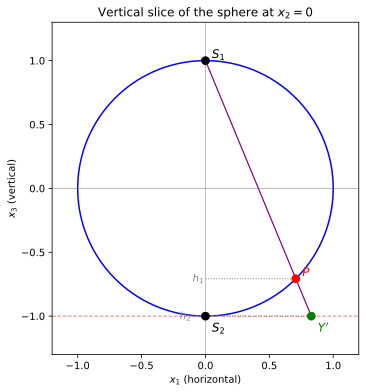
\includegraphics[width=\textwidth]{images/CircleSection.jpg}
\end{subfigure}
\hfill
\begin{subfigure}{0.48\textwidth}
    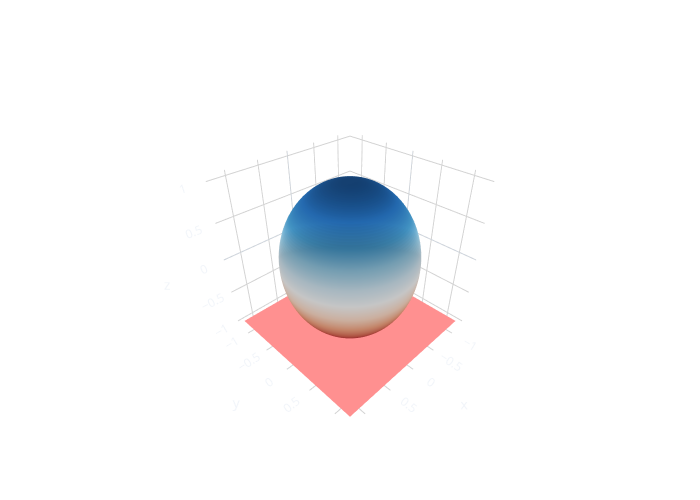
\includegraphics[width=\textwidth]{images/SpherePlane.jpg}
\end{subfigure}
\end{figure}
\begin{itemize}
    \item \textbf{Chart 1 $(U_N, \phi_N)$:} $U_N$ is the entire sphere \emph{except} the North Pole $N=(0,0,1)$. The map $\phi_N$ projects any point $P=(x^1, x^2, x^3)$ from $N$ onto the equatorial plane $x^3=-1$. The coordinates are $y^i = (y^1, y^2)$.
    The map $\phi_N$ projects from $N$ to the plane $x^3 = -1$. The coordinates are $(y^1, y^2)$. By similar triangles, the map is:
    \begin{equation}
        (y^1, y^2) = \phi_N(x^1, x^2, x^3) = \left( \frac{2x^1}{1-x^3}, \frac{2x^2}{1-x^3} \right)
    \end{equation}

    \item \textbf{Chart 2 $(U_S, \phi_S)$:} $U_S$ is the entire sphere \emph{except} the South Pole $S=(0,0,-1)$. The map $\phi_S$ projects from $S$ onto the plane $x^3 = +1$. The coordinates are $(z^1, z^2)$.
    \begin{equation}
        (z^1, z^2) = \phi_S(x^1, x^2, x^3) = \left( \frac{2x^1}{1+x^3}, \frac{2x^2}{1+x^3} \right)
    \end{equation}
\end{itemize}
These two charts co ver the entire sphere. On their overlap (the sphere minus both poles), we must check that the transition map is $C^\infty$.

\subsubsection*{Derivation: Transition Map for $S^2$}
We need to find the map $\phi_S \circ \phi_N^{-1}$, which takes coordinates $(y^1, y^2)$ from the first chart and gives the corresponding coordinates $(z^1, z^2)$ in the second chart.

\begin{enumerate}
    \item \textbf{Invert $\phi_N$:} We must find $(x^1, x^2, x^3)$ in terms of $(y^1, y^2)$.
    Let $Y^2 = (y^1)^2 + (y^2)^2$.
    \[
        Y^2 = \frac{4(x^1)^2 + 4(x^2)^2}{(1-x^3)^2}
    \]
    Using $(x^1)^2 + (x^2)^2 = 1 - (x^3)^2 = (1-x^3)(1+x^3)$:
    \[
        Y^2 = \frac{4(1-x^3)(1+x^3)}{(1-x^3)^2} = \frac{4(1+x^3)}{1-x^3}
    \]
    We can solve this for $x^3$:
    \[
        Y^2(1-x^3) = 4(1+x^3) \implies Y^2 - Y^2 x^3 = 4 + 4x^3
    \]
    \[
        Y^2 - 4 = (Y^2 + 4)x^3 \implies x^3 = \frac{Y^2 - 4}{Y^2 + 4}
    \]
    Now we find $x^1$ and $x^2$. First, find the term $(1-x^3)$:
    \[
        1 - x^3 = 1 - \frac{Y^2 - 4}{Y^2 + 4} = \frac{(Y^2 + 4) - (Y^2 - 4)}{Y^2 + 4} = \frac{8}{Y^2 + 4}
    \]
    From the definition $y^1 = 2x^1 / (1-x^3)$:
    \[
        x^1 = \frac{y^1 (1-x^3)}{2} = \frac{y^1}{2} \left( \frac{8}{Y^2 + 4} \right) = \frac{4y^1}{Y^2 + 4}
    \]
    Similarly, $x^2 = \frac{4y^2}{Y^2 + 4}$.
    This completes the inverse map $\phi_N^{-1}: (y^1, y^2) \mapsto (x^1, x^2, x^3)$.

    \item \textbf{Apply $\phi_S$:} Now we apply the second chart's map to these expressions.
    \[
        (z^1, z^2) = \left( \frac{2x^1}{1+x^3}, \frac{2x^2}{1+x^3} \right)
    \]
    We need the term $(1+x^3)$:
    \[
        1 + x^3 = 1 + \frac{Y^2 - 4}{Y^2 + 4} = \frac{(Y^2 + 4) + (Y^2 - 4)}{Y^2 + 4} = \frac{2Y^2}{Y^2 + 4}
    \]
    Now substitute:
    \[
        z^1 = \frac{2 \left( \frac{4y^1}{Y^2 + 4} \right)}{ \left( \frac{2Y^2}{Y^2 + 4} \right) } = \frac{8y^1}{2Y^2} = \frac{4y^1}{(y^1)^2 + (y^2)^2}
    \]
    \[
        z^2 = \frac{2 \left( \frac{4y^2}{Y^2 + 4} \right)}{ \left( \frac{2Y^2}{Y^2 + 4} \right) } = \frac{8y^2}{2Y^2} = \frac{4y^2}{(y^1)^2 + (y^2)^2}
    \]
\end{enumerate}
The transition map is:
\begin{equation}
    (z^1, z^2) = \left( \frac{4y^1}{(y^1)^2 + (y^2)^2}, \frac{4y^2}{(y^1)^2 + (y^2)^2} \right)
\end{equation}
This map is $C^\infty$ (smooth) everywhere except at $(y^1, y^2) = (0,0)$. This point corresponds to the South Pole, which is explicitly \emph{excluded} from the domain of $\phi_N$. Therefore, the transition map is smooth on the entire overlap region, and our two charts form a valid $C^\infty$ atlas for $S^2$.

\subsection*{The Chain Rule}
We will frequently use the chain rule for maps between coordinate patches.
% 
% 
% 
% 
% 
% 
% 
% 
% FIGURE: Carroll's Figure 2.17. Maps $f: R^m \to R^n$ and $g: R^n \to R^l$.
% 
% 
% 
% 
% 
% 
% 
If we have maps $f: \mathbb{R}^m \to \mathbb{R}^n$ and $g: \mathbb{R}^n \to \mathbb{R}^l$, with coordinates $x^a \in \mathbb{R}^m$, $y^b \in \mathbb{R}^n$, and $z^c \in \mathbb{R}^l$, the chain rule relates the partial derivatives:
\begin{equation}
    \frac{\partial (g \circ f)^c}{\partial x^a} = \sum_{b=1}^n \frac{\partial f^b}{\partial x^a} \frac{\partial g^c}{\partial y^b}
\end{equation}
A common shorthand for this operation on a function is:
\begin{equation}
    \frac{\partial}{\partial x^a} = \sum_{b=1}^n \frac{\partial y^b}{\partial x^a} \frac{\partial}{\partial y^b}
\end{equation}

\section{Vectors Again}

Having established the concept of a manifold, we must redefine our physical objects (vectors, tensors) to live on this new structure. In Chapter 1, we introduced the \textbf{tangent space} $T_p$ as the set of all vectors at a single point $p$. This was to break the (false) intuition of vectors stretching between different points. Now, we must provide a rigorous, intrinsic definition of $T_p$ that doesn't rely on embedding the manifold in a higher-dimensional space.

A natural first guess is to define $T_p$ as the set of all "tangent vectors" to all possible curves $\gamma(\lambda)$ that pass through $p$. The problem is that this is circular; we haven't yet defined what a "tangent vector" is. In a coordinate system $x^\mu$, the components $dx^\mu/d\lambda$ are coordinate-dependent and don't represent the invariant geometric object we're after.

The solution is to notice that any curve $\gamma(\lambda)$ through $p$ defines a \textbf{directional derivative operator}, $d/d\lambda$, which acts on any smooth scalar function $f: M \to \mathbb{R}$ (a space we call $\mathcal{F}$) to produce a real number:
\[
    \frac{d}{d\lambda} (f) \in \mathbb{R}
\]
We will therefore \emph{define} the tangent space $T_p$ as the set of all such directional derivative operators at $p$.

\subsection*{Vectors as Derivative Operators}
To show this is a valid definition, we must first establish that this set of operators forms a vector space.

\textbf{1. Linearity:} We can add two such operators and scale them by real numbers $a, b$:
\[
    X = a \frac{d}{d\lambda_1} + b \frac{d}{d\lambda_2}
\]
This new operator $X$ is clearly linear in its action on functions.

\textbf{2. Leibniz Rule:} A "good" derivative operator must also obey the product rule (Leibniz's rule). We can check this:
\begin{align*}
    X(fg) &= \left(a \frac{d}{d\lambda_1} + b \frac{d}{d\lambda_2}\right) (fg) \\
    &= a \left( f \frac{dg}{d\lambda_1} + g \frac{df}{d\lambda_1} \right) + b \left( f \frac{dg}{d\lambda_2} + g \frac{df}{d\lambda_2} \right) \\
    &= f \left( a \frac{dg}{d\lambda_1} + b \frac{dg}{d\lambda_2} \right) + g \left( a \frac{df}{d\lambda_1} + b \frac{df}{d\lambda_2} \right) \\
    &= f (X(g)) + g (X(f))
\end{align*}
The product rule is satisfied. Thus, the set of all such operators at $p$ forms a vector space, which we identify as the tangent space $T_p$.

\subsection*{The Coordinate Basis}
Now that $T_p$ is defined, we can find a basis for it. Given a coordinate chart with coordinates $x^\mu$ (where $\mu = 0, \dots, n-1$), there is a natural set of $n$ directional derivatives: the \textbf{partial derivative operators} $\{\partial_\mu\} \equiv \{\frac{\partial}{\partial x^\mu}\}$.
% 
% 
% 
% 
% 
% 
% 
% 
% 
% FIGURE: Carroll's Figure 2.18. A curved 2D surface with coordinate lines $x^1, x^2$. At point p, two vectors $\partial_1$ and $\partial_2$ are shown, tangent to the coordinate lines.
% 
% 
% 
% 
% 
% 
% 
% 
% 
These operators form a basis for $T_p$. To prove this, we show that any arbitrary directional derivative $d/d\lambda$ (representing any vector $V$) can be written as a unique linear combination of these partials.

\textbf{Derivation: Vector Components}
Let's assume $\phi : M \rightarrow \mathbb{R}^n$ is our coordinate chart, mapping point $p$ to coordinates $x^\mu(p)$. A curve $\gamma : \mathbb{R} \rightarrow M$ and function $f : M \rightarrow \mathbb{R}$.

\begin{equation}
\begin{split}
    \frac{d}{d\lambda}(f) &= \frac{d}{d\lambda} (f \circ \gamma) \\
    &= \frac{d}{d\lambda} [(f \circ \phi^{-1}) \circ (\phi \circ \gamma)] \\
    &= \frac{d(\phi \circ \gamma)^\mu}{d\lambda} \ \ \frac{\partial(f \circ \phi^{-1})}{\partial x^\mu} \\
    &= \frac{dx^\mu}{d\lambda} \frac{\partial f}{\partial x^\mu}
\end{split}
\end{equation}
so finally we have: 
$$\frac{d}{d\lambda} = \frac{dx^\mu}{d\lambda} {\partial_\mu }$$
\textbf{Physical Meaning:} This is a profound result. It shows that any vector $V$ (represented by $d/d\lambda$) can be written in the basis $V = V^\mu \hat{e}_{(\mu)}$ where the basis vectors are the partial derivatives $\hat{e}_{(\mu)} = \partial_\mu$ and the components $V^\mu$ are precisely the familiar $dx^\mu/d\lambda$.

This basis $\{\partial_\mu\}$ is called the \textbf{coordinate basis}. It is simple and natural, but it is crucial to remember that it is generally \emph{not} an orthonormal basis.

\subsection*{Transformation Properties}
This abstract definition makes deriving transformation laws trivial.
\begin{itemize}
    \item \textbf{Basis Vector Transformation:} How does the basis $\{\partial_\mu\}$ change when we change coordinates from $x^\mu$ to $x^{\mu'}$? The new basis vectors $\partial_{\mu'} \equiv \frac{\partial}{\partial x^{\mu'}}$ are related to the old ones by the chain rule:
    \begin{equation}
        \partial_{\mu'} = \frac{\partial}{\partial x^{\mu'}} = \frac{\partial x^\mu}{\partial x^{\mu'}} \frac{\partial}{\partial x^\mu} = \frac{\partial x^\mu}{\partial x^{\mu'}} \partial_\mu
    \end{equation}
    This is the transformation law for the basis vectors.

    \item \textbf{Vector Component Transformation:} The abstract vector $V$ itself is invariant to coordinate choice. Its expansion in either basis must be equal:
    \[
        V = V^{\mu'} \partial_{\mu'} = V^\mu \partial_\mu
    \]
    Substituting the basis transformation:
    \[
        V = V^{\mu'} \left( \frac{\partial x^\mu}{\partial x^{\mu'}} \partial_\mu \right)
    \]
    By comparing this to $V = V^\mu \partial_\mu$, and since the $\{\partial_\mu\}$ are a basis, the coefficients must be equal:
    \[
        V^\mu = V^{\mu'} \frac{\partial x^\mu}{\partial x^{\mu'}}
    \]
    To find the transformation for $V^{\mu'}$, we just invert this relationship using the inverse Jacobian matrix:
    \begin{equation}
        V^{\mu'} = \frac{\partial x^{\mu'}}{\partial x^\mu} V^\mu
    \end{equation}
    This is the familiar transformation law for a contravariant vector, but now derived for \emph{any} smooth coordinate change, not just the linear Lorentz transformations of flat space.
\end{itemize}
% 
% 
% 
% 
% 
% 
% 
% FIGURE: Carroll's Figure 2.20. A manifold patch shown with two different coordinate grids ($x^\mu$ and $x^{\mu'}$), and their respective (non-parallel, non-orthogonal) basis vectors $\partial_\mu$ and $\partial_{\mu'}$.
% 
% 
% 
% 
% 
% 
% 
\subsection*{The Commutator (Lie Bracket)}
A vector field $X = X^\mu(x) \partial_\mu$ is an operator that maps scalar fields to scalar fields ($X: \mathcal{F} \to \mathcal{F}$). This allows us to define the \textbf{commutator} (or \textbf{Lie bracket}) of two vector fields, $X$ and $Y$, by its action on an arbitrary scalar field $f$:
\begin{equation}
    [X, Y](f) \equiv X(Y(f)) - Y(X(f))
\end{equation}
Crucially, the resulting object $[X, Y]$ is \emph{also} a vector field, meaning it is a linear, first-order differential operator that obeys the Leibniz rule.

\textbf{Derivation: Component Form of the Commutator}
We can find the components of the vector field $Z = [X, Y]$ in a coordinate basis. The $\nu$-th component $Z^\nu$ can be found by acting the operator on the coordinate function $x^\nu$ (since $Z(x^\nu) = Z^\mu \partial_\mu x^\nu = Z^\mu \delta^\nu_\mu = Z^\nu$).
\begin{align*}
    [X, Y]^\nu &= [X, Y](x^\nu) \\
    &= X(Y(x^\nu)) - Y(X(x^\nu)) \\
    &= X(Y^\mu \partial_\mu x^\nu) - Y(X^\lambda \partial_\lambda x^\nu) \\
    &= X(Y^\mu \delta^\nu_\mu) - Y(X^\lambda \delta^\nu_\lambda) \\
    &= X(Y^\nu) - Y(X^\nu) \\
    &= (X^\lambda \partial_\lambda) Y^\nu - (Y^\mu \partial_\mu) X^\nu
\end{align*}
By renaming the dummy index $\mu$ to $\lambda$ in the second term, we get the standard expression:
\begin{equation}
    [X, Y]^\nu = X^\lambda \partial_\lambda Y^\nu - Y^\lambda \partial_\lambda X^\nu
\end{equation}
It may seem surprising that this is a well-defined tensor, since it involves partial derivatives of vector components, which are not themselves tensors. However, the non-tensorial "extra pieces" that arise in a coordinate transformation of the first term ($\partial_\lambda Y^\nu$) are precisely canceled by those from the second term ($\partial_\lambda X^\nu$), leaving a valid tensor transformation law.

A simple, important example is the commutator of two coordinate basis vectors:
\[
    [\partial_\mu, \partial_\nu](f) = \partial_\mu(\partial_\nu f) - \partial_\nu(\partial_\mu f) = 0
\]
This is a direct consequence of the fact that partial derivatives commute.
\section{Tensors Again}

With a rigorous definition of vectors and the tangent space $T_p$, we can retrace our steps from Chapter 1 to define dual vectors (one-forms) and, more generally, tensors on a manifold.

\subsection*{Dual Vectors (One-Forms)}
The \textbf{cotangent space} $T_p^*$ is defined as the dual vector space to $T_p$. That is, $T_p^*$ is the set of all linear maps $\omega: T_p \to \mathbb{R}$.

The canonical example of a one-form is the \textbf{gradient} of a scalar function $f$, denoted $df$. Its "action" on a vector $V$ is defined to be the directional derivative of $f$ along $V$:
\[
    df(V) \equiv V(f)
\]
If we use our definition of a vector $V$ as the tangent vector to a curve $x^\mu(\lambda)$, $V = d/d\lambda$, then its action is just the ordinary derivative:
\begin{equation}
    df\left(\frac{d}{d\lambda}\right) = \frac{df}{d\lambda}
\end{equation}

\subsection*{Basis and Components}
Just as the partial derivatives $\{\partial_\mu\}$ form a natural basis for the tangent space $T_p$, the gradients of the coordinate functions $\{dx^\mu\}$ form a natural basis for the cotangent space $T_p^*$.

We can prove this by showing that $\{dx^\mu\}$ is the \textbf{dual basis} to $\{\partial_\nu\}$, which means their "action" on each other is the Kronecker delta.
\begin{enumerate}
    \item Start with the definition of the action of the one-form $dx^\mu$ on the vector $\partial_\nu$:
    \[
        dx^\mu (\partial_\nu) \equiv \partial_\nu (x^\mu)
    \]
    \item The partial derivative of the coordinate function $x^\mu$ with respect to the coordinate $x^\nu$ is:
    \[
        \partial_\nu (x^\mu) = \frac{\partial x^\mu}{\partial x^\nu} = \delta^\mu_\nu
    \]
\end{enumerate}
Thus, we have our duality relationship:
\begin{equation}
    dx^\mu (\partial_\nu) = \delta^\mu_\nu
\end{equation}
Any arbitrary one-form $\omega$ can be expanded in this basis using its components $\omega_\mu$:
\[
    \omega = \omega_\mu dx^\mu
\]

\subsection*{Transformation Properties}
The transformation laws follow directly from the chain rule.
\begin{itemize}
    \item \textbf{Basis One-Forms:} The new basis one-forms $dx^{\mu'}$ are related to the old $dx^\mu$ by the standard rule for total differentials:
    \begin{equation}
        dx^{\mu'} = \frac{\partial x^{\mu'}}{\partial x^\mu} dx^\mu
    \end{equation}
    \item \textbf{Components:} The components $\omega_\mu$ must transform in the "opposite" (inverse) way to keep the abstract one-form $\omega$ invariant.
    \[
        \omega = \omega_\mu dx^\mu = \omega_{\mu'} dx^{\mu'}
    \]
    Substituting the basis transformation:
    \[
        \omega = \omega_{\mu'} \left( \frac{\partial x^{\mu'}}{\partial x^\mu} dx^\mu \right)
    \]
    By matching the $dx^\mu$ components, we find $\omega_\mu = \omega_{\mu'} \frac{\partial x^{\mu'}}{\partial x^\mu}$. We can invert this by multiplying by $\frac{\partial x^\mu}{\partial x^{\nu'}}$ to get the standard form:
    \begin{equation}
        \omega_{\nu'} = \frac{\partial x^\mu}{\partial x^{\nu'}} \omega_\mu
    \end{equation}
\end{itemize}

\subsection*{General Tensors}
A tensor $T$ of type (or rank) $(k, l)$ is a multilinear map from $k$ copies of the cotangent space and $l$ copies of the tangent space to the real numbers:
\[
    T: \underbrace{T_p^* \times \dots \times T_p^*}_{k \text{ times}} \times \underbrace{T_p \times \dots \times T_p}_{l \text{ times}} \to \mathbb{R}
\]
In a coordinate basis, any tensor can be expanded using its components:
\begin{equation}
    T = {T^{\mu_1 \dots \mu_k}}_{\nu_1 \dots \nu_l} \partial_{\mu_1} \otimes \dots \otimes \partial_{\mu_k} \otimes dx^{\nu_1} \otimes \dots \otimes dx^{\nu_l}
\end{equation}
The components are found by acting the tensor on the basis vectors and one-forms:
\begin{equation}
    {T^{\mu_1 \dots \mu_k}}_{\nu_1 \dots \nu_l} = T(dx^{\mu_1}, \dots, dx^{\mu_k}, \partial_{\nu_1}, \dots, \partial_{\nu_l})
\end{equation}
The general \textbf{tensor transformation law} replaces the Lorentz matrices from Chapter 1 with the more general Jacobian matrices of the coordinate transformation. Each index transforms according to its type (contravariant or covariant):
\begin{equation}
    {T^{\mu'_1 \dots \mu'_k}}_{\nu'_1 \dots \nu'_l} = 
    \underbrace{
    \frac{\partial x^{\mu'_1}}{\partial x^{\mu_1}} \dots \frac{\partial x^{\mu'_k}}{\partial x^{\mu_k}}
    }_{\text{contravariant indices}}
    \underbrace{
    \frac{\partial x^{\nu_1}}{\partial x^{\nu'_1}} \dots \frac{\partial x^{\nu_l}}{\partial x^{\nu'_l}}
    }_{\text{covariant indices}}
    {T^{\mu_1 \dots \mu_k}}_{\nu_1 \dots \nu_l}
\end{equation}

\subsection*{Example: Transforming a (0,2) Tensor}
Applying the full transformation law (2.30) is cumbersome. It is often much simpler to transform a tensor by transforming its basis vectors and one-forms directly.

Let's consider a symmetric (0,2) tensor $S$ on a 2D manifold with coordinates $(x^1, x^2) = (x, y)$. In this frame, $S$ has components:
\[
    S_{\mu\nu} = \begin{pmatrix} 1 & 0 \\ 0 & x^2 \end{pmatrix}
\]
As an abstract tensor, this is written (suppressing the $\otimes$ symbol):
\begin{equation}
    S = S_{\mu\nu} dx^\mu dx^\nu = 1 \, (dx)^2 + x^2 (dy)^2
\end{equation}
Now, let's change to a new coordinate system $(x', y')$ defined by:
\[
    x' = \frac{2x}{y}, \quad y' = \frac{y}{2}
\]
\textbf{Derivation:}
\begin{enumerate}
    \item \textbf{Invert the transformation} to express old coordinates in terms of new:
    \[
        y = 2y'
    \]
    \[
        x = \frac{x' y}{2} = \frac{x' (2y')}{2} = x'y'
    \]
    \item \textbf{Find the old basis one-forms} in terms of the new ones by differentiation:
    \[
        dx = \frac{\partial x}{\partial x'} dx' + \frac{\partial x}{\partial y'} dy' = y' dx' + x' dy'
    \]
    \[
        dy = \frac{\partial y}{\partial x'} dx' + \frac{\partial y}{\partial y'} dy' = 0 \, dx' + 2 dy' = 2 dy'
    \]
    \item \textbf{Substitute} these expressions directly into the abstract tensor $S$:
    \[
        S = (y'dx' + x'dy')^2 + (x'y')^2 (2dy')^2
    \]
    We must be careful to treat $dx'dy'$ as $dx' \otimes dy'$:
    \[
        S = (y'dx' + x'dy') \otimes (y'dx' + x'dy') + (x'y')^2 (2dy' \otimes 2dy')
    \]
    \item \textbf{Expand} the tensor products:
    \[
        S = (y')^2 (dx' \otimes dx') + x'y' (dx' \otimes dy') + x'y' (dy' \otimes dx') + (x')^2 (dy' \otimes dy') + 4(x'y')^2 (dy' \otimes dy')
    \]
    \item \textbf{Combine} terms (and revert to the $dx'dy'$ shorthand, remembering it's symmetric):
    \[
        S = (y')^2 (dx')^2 + x'y' (dx'dy' + dy'dx') + \left[ (x')^2 + 4(x'y')^2 \right] (dy')^2
    \]
\end{enumerate}
By reading off the components $S = S_{\mu'\nu'} dx^{\mu'} dx^{\nu'}$, we find the new component matrix:
\begin{equation} \label{S_transform}
    S_{\mu'\nu'} = \begin{pmatrix}
        (y')^2 & x'y' \\
        x'y' & (x')^2 + 4(x'y')^2
    \end{pmatrix}
\end{equation}
This matches the result one would get from the full transformation law (2.30), but was much easier to derive.

\begin{equation}
    S_{\mu'\nu'} = \frac{\partial x^\mu}{\partial x^{\mu'}} \ \frac{\partial x^\nu}{\partial x^{\nu'}} \, S_{\mu \nu}
\end{equation}
First we calculate the partial derivatives:
$$\frac{\partial x}{\partial x'} = y', \quad \frac{\partial x}{\partial y'} = x', \quad \frac{\partial y}{\partial x'} = 0, \quad \frac{\partial y}{\partial y'} = 2$$
So now we can compute each component:
\begin{align*}
    S_{x'x'} &= \frac{\partial x}{\partial x'} \frac{\partial x}{\partial x'} S_{xx} + \frac{\partial x}{\partial x'} \frac{\partial y}{\partial x'} S_{xy} + \frac{\partial y}{\partial x'} \frac{\partial x}{\partial x'} S_{yx} + \frac{\partial y}{\partial x'} \frac{\partial y}{\partial x'} S_{yy} \\
    &= (y')(y')(1) + (y')(0)(0) + (0)(y')(0) + (0)(0)(x^2) = (y')^2 \\
    S_{x'y'} &= \frac{\partial x}{\partial x'} \frac{\partial x}{\partial y'} S_{xx} + \frac{\partial x}{\partial x'} \frac{\partial y}{\partial y'} S_{xy} + \frac{\partial y}{\partial x'} \frac{\partial x}{\partial y'} S_{yx} + \frac{\partial y}{\partial x'} \frac{\partial y}{\partial y'} S_{yy} \\
    &= (y')(x')(1) + (y')(2)(0) + (0)(x')(0) + (0)(2)(x^2) = x'y' \\
    S_{y'y'} &= \frac{\partial x}{\partial y'} \frac{\partial x}{\partial y'} S_{xx} + \frac{\partial x}{\partial y'} \frac{\partial y}{\partial y'} S_{xy} + \frac{\partial y}{\partial y'} \frac{\partial x}{\partial y'} S_{yx} + \frac{\partial y}{\partial y'} \frac{\partial y}{\partial y'} S_{yy} \\
    &= (x')(x')(1) + (x')(2)(0) + (2)(x')(0) + (2)(2)(x^2) = (x')^2 + 4(x'y')^2
\end{align*} 

which give us the equation (\ref{S_transform}) again.
\subsection*{The Failure of Partial Derivatives}
In Chapter 1, we noted that in flat space with \emph{inertial} coordinates, the partial derivative of a tensor was also a tensor. This property \textbf{fails} in a general manifold (or even in flat space with curvilinear coordinates).

The partial derivative of a scalar $\partial_\mu \phi$ is a valid (0,1) tensor (a one-form).
However, the partial derivative of a vector $\partial_\mu V^\nu$ or a one-form $\partial_\mu W_\nu$ is \textbf{not a tensor}.

\textbf{Proof (for a one-form):}
Let's see what happens when we try to transform the components of $\partial_\mu W_\nu$ to the new $x'$ frame. The object we are transforming is $K_{\mu\nu} = \partial_\mu W_\nu$. The transformed components would be $K_{\mu'\nu'} = \partial_{\mu'} W_{\nu'}$.
\begin{enumerate}
    \item Start with the transformed object $\partial_{\mu'} W_{\nu'}$.
    \[
        \partial_{\mu'} W_{\nu'} = \frac{\partial}{\partial x^{\mu'}} \left( W_{\nu'} \right)
    \]
    \item Substitute the transformation law for the one-form component $W_{\nu'}$:
    \[
        \partial_{\mu'} W_{\nu'} = \frac{\partial}{\partial x^{\mu'}} \left( \frac{\partial x^\nu}{\partial x^{\nu'}} W_\nu \right)
    \]
    \item Apply the product rule (since both $\frac{\partial x^\nu}{\partial x^{\nu'}}$ and $W_\nu$ are functions of position):
    \[
        \partial_{\mu'} W_{\nu'} = \left( \frac{\partial}{\partial x^{\mu'}} \frac{\partial x^\nu}{\partial x^{\nu'}} \right) W_\nu + \frac{\partial x^\nu}{\partial x^{\nu'}} \left( \frac{\partial}{\partial x^{\mu'}} W_\nu \right)
    \]
    \item Apply the chain rule to both terms:
    \[
        \partial_{\mu'} W_{\nu'} = \underbrace{ \left( \frac{\partial x^\mu}{\partial x^{\mu'}} \frac{\partial^2 x^\nu}{\partial x^\mu \partial x^{\nu'}} \right) W_\nu }_{\text{Term 1}} + \underbrace{ \frac{\partial x^\nu}{\partial x^{\nu'}} \left( \frac{\partial x^\mu}{\partial x^{\mu'}} \frac{\partial}{\partial x^\mu} W_\nu \right) }_{\text{Term 2}}
    \]
\end{enumerate}
Rearranging the terms, we get:
\begin{equation}
    \partial_{\mu'} W_{\nu'} = 
    \underbrace{
    \frac{\partial x^\mu}{\partial x^{\mu'}} \frac{\partial x^\nu}{\partial x^{\nu'}} (\partial_\mu W_\nu)
    }_{\text{This is the correct tensor transformation...}}
    +
    \underbrace{
    W_\nu \frac{\partial^2 x^\nu}{\partial x^{\mu'} \partial x^{\nu'}}
    }_{\text{...but this extra "bad" term is not zero!}}
\end{equation}
This "bad" second term arises from the derivative of the transformation matrix itself. It is zero \emph{only if} the transformation is linear (all second derivatives $\frac{\partial^2 x}{\partial x' \partial x'}$ are zero), as is the case for Lorentz transformations. For a general coordinate change, this term is non-zero, and $\partial_\mu W_\nu$ fails to transform as a (0,2) tensor.

This fundamental problem is the primary motivation for introducing a new, more powerful type of derivative that \emph{is} a tensor: the \textbf{covariant derivative}.

\section{The Metric}

The metric tensor, now denoted $g_{\mu\nu}$, is the central object in general relativity. It is a symmetric, (0,2) tensor field that endows the manifold with a notion of distance, time, and causal structure.

We will almost always assume the metric is \textbf{nondegenerate}, meaning its determinant $g = \det(g_{\mu\nu})$ is non-zero. This ensures that an inverse metric $g^{\mu\nu}$ exists, which is defined by the relation:
\begin{equation}
    g^{\mu\nu} g_{\nu\sigma} = \delta^\mu_\sigma
\end{equation}
The metric and its inverse are the tools we use to raise and lower indices on all other tensors (e.g., $V_\mu = g_{\mu\nu} V^\nu$).

The metric $g_{\mu\nu}$ plays numerous roles, including:
\begin{itemize}
    \item Defining the causal structure (past, future, light cones).
    \item Allowing the computation of proper time and path lengths.
    \item Determining the "shortest paths" (geodesics) on which test particles move.
    \item Replacing the single Newtonian potential $\Phi$.
    \item Defining locally inertial frames and thus a notion of "no rotation."
    \item Determining the speed of light and causality.
    \item Replacing the 3D Euclidean dot product.
\end{itemize}

\subsection*{The Line Element}
As in flat space, we write the metric in the form of the \textbf{line element}, $ds^2$. This is a convenient shorthand for the abstract (0,2) tensor $g$:
\begin{equation}
    ds^2 = g_{\mu\nu} dx^\mu dx^\nu
\end{equation}
Here, the $dx^\mu$ are formally understood as the basis one-forms. The inner product of two vectors $V$ and $W$ is $g(V, W) = g_{\mu\nu}V^\mu W^\nu$.

\subsection*{Example: Flat Space in Spherical Coordinates}
The metric components $g_{\mu\nu}$ depend on the coordinate system. Even flat Euclidean space has non-trivial metric components in curvilinear coordinates.
The Cartesian line element for flat 3D space is $ds^2 = (dx)^2 + (dy)^2 + (dz)^2$.
The transformation to spherical coordinates $(r, \theta, \phi)$ is:
\begin{align*}
    x &= r \sin\theta \cos\phi \\
    y &= r \sin\theta \sin\phi \\
    z &= r \cos\theta
\end{align*}

\textbf{Derivation:}
We find the new metric by calculating the differentials $dx$, $dy$, and $dz$ and substituting them into the Cartesian line element.
\begin{enumerate}
    \item \textbf{Calculate the differentials} using the multivariable chain rule:
    \begin{align*}
        dx &= (\sin\theta\cos\phi)dr + (r\cos\theta\cos\phi)d\theta - (r\sin\theta\sin\phi)d\phi \\
        dy &= (\sin\theta\sin\phi)dr + (r\cos\theta\sin\phi)d\theta + (r\sin\theta\cos\phi)d\phi \\
        dz &= (\cos\theta)dr - (r\sin\theta)d\theta
    \end{align*}
    \item \textbf{Square the differentials.} We must compute $(dx)^2 + (dy)^2 + (dz)^2$. This is tedious, but many cross-terms will cancel. Let's first compute $(dx)^2 + (dy)^2$:
    \begin{align*}
        (dx)^2 &= (\sin^2\theta\cos^2\phi)dr^2 + (r^2\cos^2\theta\cos^2\phi)d\theta^2 + (r^2\sin^2\theta\sin^2\phi)d\phi^2 \\
                &+ 2(r\sin\theta\cos\theta\cos^2\phi)dr d\theta - 2(r\sin^2\theta\sin\phi\cos\phi)dr d\phi \\
                &- 2(r^2\sin\theta\cos\theta\sin\phi\cos\phi)d\theta d\phi \\
        \\
        (dy)^2 &= (\sin^2\theta\sin^2\phi)dr^2 + (r^2\cos^2\theta\sin^2\phi)d\theta^2 + (r^2\sin^2\theta\cos^2\phi)d\phi^2 \\
                &+ 2(r\sin\theta\cos\theta\sin^2\phi)dr d\theta + 2(r\sin^2\theta\sin\phi\cos\phi)dr d\phi \\
                &+ 2(r^2\sin\theta\cos\theta\sin\phi\cos\phi)d\theta d\phi
    \end{align*}
    \item \textbf{Sum $(dx)^2 + (dy)^2$} by collecting terms and using $\cos^2\phi + \sin^2\phi = 1$:
    \begin{itemize}
        \item $dr^2$ term: $(\sin^2\theta\cos^2\phi + \sin^2\theta\sin^2\phi)dr^2 = \sin^2\theta dr^2$
        \item $d\theta^2$ term: $(r^2\cos^2\theta\cos^2\phi + r^2\cos^2\theta\sin^2\phi)d\theta^2 = r^2\cos^2\theta d\theta^2$
        \item $d\phi^2$ term: $(r^2\sin^2\theta\sin^2\phi + r^2\sin^2\theta\cos^2\phi)d\phi^2 = r^2\sin^2\theta d\phi^2$
        \item $dr d\theta$ term: $2(r\sin\theta\cos\theta(\cos^2\phi + \sin^2\phi))dr d\theta = 2r\sin\theta\cos\theta dr d\theta$
        \item $dr d\phi$ term: The cross terms cancel to 0.
        \item $d\theta d\phi$ term: The cross terms cancel to 0.
    \end{itemize}
    So, $(dx)^2 + (dy)^2 = \sin^2\theta dr^2 + r^2\cos^2\theta d\theta^2 + r^2\sin^2\theta d\phi^2 + 2r\sin\theta\cos\theta dr d\theta$.
    
    \item \textbf{Now add $(dz)^2$:}
    \[
        (dz)^2 = (\cos\theta dr - r\sin\theta d\theta)^2 = \cos^2\theta dr^2 - 2r\sin\theta\cos\theta dr d\theta + r^2\sin^2\theta d\theta^2
    \]
    \item \textbf{Sum all three parts:}
    \begin{align*}
        ds^2 &= \left[ (dx)^2 + (dy)^2 \right] + (dz)^2 \\
             &= \left[ \sin^2\theta dr^2 + r^2\cos^2\theta d\theta^2 + r^2\sin^2\theta d\phi^2 + 2r\sin\theta\cos\theta dr d\theta \right] \\
             & \quad + \left[ \cos^2\theta dr^2 - 2r\sin\theta\cos\theta dr d\theta + r^2\sin^2\theta d\theta^2 \right]
    \end{align*}
    \item \textbf{Collect final terms:}
    \begin{itemize}
        \item $dr^2$ term: $(\sin^2\theta + \cos^2\theta)dr^2 = dr^2$
        \item $d\theta^2$ term: $(r^2\cos^2\theta + r^2\sin^2\theta)d\theta^2 = r^2 d\theta^2$
        \item $d\phi^2$ term: $r^2\sin^2\theta d\phi^2$
        \item $dr d\theta$ term: $(2r\sin\theta\cos\theta - 2r\sin\theta\cos\theta) dr d\theta = 0$
    \end{itemize}
\end{enumerate}
The final result is the metric for flat 3D space in spherical coordinates:
\begin{equation}
    ds^2 = dr^2 + r^2 d\theta^2 + r^2\sin^2\theta d\phi^2
\end{equation}
From this, we can read off the non-zero metric components: $g_{rr}=1$, $g_{\theta\theta}=r^2$, and $g_{\phi\phi}=r^2\sin^2\theta$. This metric is for a \emph{flat} space, even though its components depend on the coordinates $r$ and $\theta$. Curvature is a more subtle concept.

\subsection*{Example: The 2-Sphere $S^2$}
We can find the metric of a 2-dimensional sphere of radius $R$ by taking the 3D spherical metric, setting $r=R$ (a constant), and thus setting $dr=0$.
\begin{equation}
    ds^2 = R^2 d\theta^2 + R^2\sin^2\theta d\phi^2
\end{equation}
For a unit sphere ($R=1$), this is $ds^2 = d\theta^2 + \sin^2\theta d\phi^2$. This is a \emph{curved} space.
%
%
%
%
%
% FIGURE: Carroll's Figure 2.21. A small patch on a 2-sphere, showing the lengths $d\theta$ (along a longitude) and $\sin\theta d\phi$ (along a latitude) forming an infinitesimal right-triangle with hypotenuse $ds$.
%
%
%
%
%
%
\subsection*{Locally Inertial Coordinates}
The EEP states that at any point $p$ in spacetime, we can construct a \textbf{locally inertial coordinate system} (or \textbf{local Lorentz frame}) in which the laws of physics take their special relativity form.

In this frame (with hatted indices, $x^{\hat{\mu}}$), the metric at $p$ must look like the flat Minkowski metric $\eta_{\hat{\mu}\hat{\nu}}$, and any non-gravitational "forces" must vanish. This means the first derivatives of the metric must also vanish at $p$.
A coordinate system $x^{\hat{\mu}}$ is a \textbf{locally inertial coordinate (LIC)} system at $p$ if:
\begin{align}
    g_{\hat{\mu}\hat{\nu}}(p) &= \eta_{\hat{\mu}\hat{\nu}} \\
    \partial_{\hat{\sigma}} g_{\hat{\mu}\hat{\nu}}(p) &= 0
\end{align}
This is the rigorous, mathematical statement of the Equivalence Principle. We can always find coordinates where gravity "vanishes" to first order at a point.

However, we \emph{cannot} in general make the second derivatives $\partial_{\hat{\rho}}\partial_{\hat{\sigma}} g_{\hat{\mu}\hat{\nu}}(p)$ vanish. These components describe the failure of nearby locally inertial frames to be parallel; they encode the \textbf{curvature} of spacetime (tidal forces).

\textbf{Derivation (Counting Degrees of Freedom):}
We can prove this is possible by counting the number of "free parameters" we have in a coordinate transformation. In 4D ($n=4$):
\begin{enumerate}
    \item \textbf{Zeroth Order (Setting $g_{\hat{\mu}\hat{\nu}} = \eta_{\hat{\mu}\hat{\nu}}$):}
    \begin{itemize}
        \item \textbf{Components to fix:} $g_{\hat{\mu}\hat{\nu}}$ is symmetric, so it has $\frac{1}{2}n(n+1) = \frac{1}{2}(4)(5) = \textbf{10}$ independent components.
        \item \textbf{Parameters we control:} We can choose the $n \times n$ Jacobian matrix $\frac{\partial x^\mu}{\partial x^{\hat{\nu}}}$, which has $n^2 = \textbf{16}$ independent parameters.
        \item \textbf{Conclusion:} We have 16 parameters to fix 10 components. This is easily possible. (The $16 - 10 = 6$ remaining parameters are the 3 rotations and 3 boosts of the Lorentz group, which leave $\eta_{\hat{\mu}\hat{\nu}}$ unchanged).
    \end{itemize}
    \item \textbf{First Order (Setting $\partial_{\hat{\sigma}} g_{\hat{\mu}\hat{\nu}} = 0$):}
    \begin{itemize}
        \item \textbf{Components to fix:} There are $n=4$ choices for the derivative index $\hat{\sigma}$, and 10 components for $g_{\hat{\mu}\hat{\nu}}$. Total = $4 \times 10 = \textbf{40}$ components.
        \item \textbf{Parameters we control:} We can now choose the $n^3$ second derivatives $\frac{\partial^2 x^\mu}{\partial x^{\hat{\nu}} \partial x^{\hat{\sigma}}}$. This object is symmetric in its two lower indices. The number of components is $n \times \frac{1}{2}n(n+1) = 4 \times 10 = \textbf{40}$ parameters.
        \item \textbf{Conclusion:} We have exactly 40 parameters to fix 40 components. It is always possible to set the first derivatives of the metric to zero.
    \end{itemize}
    \item \textbf{Second Order (Setting $\partial_{\hat{\rho}}\partial_{\hat{\sigma}} g_{\hat{\mu}\hat{\nu}} = 0$):}
    \begin{itemize}
        \item \textbf{Components to fix:} The object $\partial_{\hat{\rho}}\partial_{\hat{\sigma}} g_{\hat{\mu}\hat{\nu}}$ is symmetric in $\hat{\mu},\hat{\nu}$ (10 components) and in $\hat{\rho},\hat{\sigma}$ (10 components). Total = $10 \times 10 = \textbf{100}$ components.
        \item \textbf{Parameters we control:} We can now choose the third derivatives $\frac{\partial^3 x^\mu}{\partial x^{\hat{\nu}} \partial x^{\hat{\sigma}} \partial x^{\hat{\rho}}}$. This is symmetric in its three lower indices.
        \item The number of independent components for 3 symmetric indices in $n=4$ dimensions is $\frac{n(n+1)(n+2)}{3!} = \frac{4 \cdot 5 \cdot 6}{6} = 20$.
        \item The total number of parameters we control is $n$ (for the $\mu$ index) $\times$ 20 = $4 \times 20 = \textbf{80}$ parameters.
        \item \textbf{Conclusion:} We have 80 parameters of freedom but need to fix 100 components. We are short by \textbf{20} components.
    \end{itemize}
\end{enumerate}
These 20 components that we \emph{cannot} set to zero by a clever choice of coordinates are the 20 independent components of the \textbf{Riemann curvature tensor}, $R_{\hat{\rho}\hat{\sigma}\hat{\mu}\hat{\nu}}$.

\subsection*{Utility of Locally Inertial Coordinates}
The existence of LICs is an incredibly powerful tool. We can solve complex problems by:
\begin{enumerate}
    \item Transforming to a LIC at the point of interest $p$.
    \item In this frame, $g_{\hat{\mu}\hat{\nu}} = \eta_{\hat{\mu}\hat{\nu}}$ and all physics reduces to Special Relativity.
    \item Solving the problem using SR.
    \item Writing the answer as a general tensor equation.
\end{enumerate}
Since a tensor equation that is true in one coordinate system is true in all, this "SR" answer is the correct, general answer for any curved spacetime.

\textbf{Example: Relative Velocity}
What is the 3-velocity $v$ of a rocket (with 4-velocity $V^\mu$) as measured by an observer (with 4-velocity $U^\mu$)?
\begin{enumerate}
    \item Go to the observer's LIC. In this frame, the observer is at rest, so $U^{\hat{\mu}} = (1, 0, 0, 0)$.
    \item The rocket's 4-velocity in this frame is $V^{\hat{\mu}} = (\gamma, \gamma v^1, \gamma v^2, \gamma v^3)$, where $v^2 = (v^1)^2 + (v^2)^2 + (v^3)^2$ and $\gamma = (1-v^2)^{-1/2}$.
    \item In this SR frame, let's compute the scalar product $g_{\hat{\mu}\hat{\nu}} U^{\hat{\mu}} V^{\hat{\nu}} = \eta_{\hat{\mu}\hat{\nu}} U^{\hat{\mu}} V^{\hat{\nu}}$:
    \[
        \eta_{\hat{\mu}\hat{\nu}} U^{\hat{\mu}} V^{\hat{\nu}} = \eta_{00} U^{\hat{0}} V^{\hat{0}} = (-1)(1)(\gamma) = -\gamma
    \]
    \item We have the SR result $\gamma = - ( \eta_{\hat{\mu}\hat{\nu}} U^{\hat{\mu}} V^{\hat{\nu}} )$.
    \item We know $\gamma = (1-v^2)^{-1/2}$, so $\gamma^{-2} = 1-v^2$, which gives $v = \sqrt{1 - \gamma^{-2}}$.
    \item Substitute our SR result for $\gamma$:
    \[
        v = \sqrt{1 - ( - \eta_{\hat{\mu}\hat{\nu}} U^{\hat{\mu}} V^{\hat{\nu}} )^{-2}} = \sqrt{1 - ( \eta_{\hat{\mu}\hat{\nu}} U^{\hat{\mu}} V^{\hat{\nu}} )^{-2}}
    \]
    \item This is a tensor equation. It must be true in \emph{any} coordinate system.
\end{enumerate}
The general, covariant expression for the relative 3-velocity is:
\begin{equation}
    v = \sqrt{1 - (g_{\mu\nu} U^\mu V^\nu)^{-2}}
\end{equation}
\section{An Expanding Universe}

A simple yet non-trivial example of a Lorentzian geometry is the flat \textbf{Robertson-Walker (RW) metric}. This metric describes a homogeneous and isotropic universe where the spatial sections (at constant time) are flat Euclidean 3-space, but the distance between points is scaled by a time-dependent \textbf{scale factor}, $a(t)$.

The line element is:
\begin{equation}\label{eq:rw-metric}
    ds^2 = -dt^2 + a^2(t)[(dx)^2 + (dy)^2 + (dz)^2]
\end{equation}
Observers who remain at constant spatial coordinates $(x, y, z)$ are called \textbf{comoving} observers. The physical distance between two comoving observers grows over time as $a(t)$.

A common set of solutions for $a(t)$ are power laws (e.g., from a Big Bang singularity at $t=0$):
\begin{equation}
    a(t) = t^q, \quad \text{for } 0 < q < 1
\end{equation}
(For example, a universe dominated by radiation has $q=1/2$, and one dominated by matter has $q=2/3$.)

\subsection*{Light Cones and Causal Structure}
The causal structure is defined by null paths ($ds^2=0$). Let's find the light cone for an observer at the origin, considering only a path in the $x-t$ plane ($dy=dz=0$). For $a(t) = t^q$, the null condition $ds^2=0$ becomes:
\[
    0 = -dt^2 + a(t)^2 (dx)^2 = -dt^2 + t^{2q} (dx)^2
\]
This implies:
\begin{equation}
    \frac{dx}{dt} = \pm t^{-q}
\end{equation}

\subsubsection*{Justifying the $dx/dt$ Notation}
The expression $\frac{dx}{dt}$ can seem "sloppy," as $dx$ and $dt$ are basis one-forms, not simple differentials. The procedure is justified by formally considering the action of the metric tensor $g$ on the tangent vector $V = \frac{dx^\mu}{d\lambda} \partial_\mu$ to a null curve $x^\mu(\lambda)$.

\begin{enumerate}
    \item The "null curve" condition is $g(V,V) = 0$.
    \begin{align*}
        g(V,V) &= g_{\mu\nu} V^\mu V^\nu \\
               &= g_{\mu\nu} \frac{dx^\mu}{d\lambda} \frac{dx^\nu}{d\lambda} \\
               &= g_{tt} \frac{dt}{d\lambda} \frac{dt}{d\lambda} + g_{xx} \frac{dx}{d\lambda} \frac{dx}{d\lambda} \quad (\text{since } dy=dz=0) \\
               &= -1 \left(\frac{dt}{d\lambda}\right)^2 + a(t)^2 \left(\frac{dx}{d\lambda}\right)^2 = 0
    \end{align*}
    \item For $a(t) = t^q$, this is:
    \begin{equation}
        -\left(\frac{dt}{d\lambda}\right)^2 + t^{2q} \left(\frac{dx}{d\lambda}\right)^2 = 0
    \end{equation}
    \item We can rearrange this to:
    \[
        \frac{\left(\frac{dx}{d\lambda}\right)^2}{\left(\frac{dt}{d\lambda}\right)^2} = \frac{1}{t^{2q}} = t^{-2q}
    \]
    \item By the standard 1D chain rule, $\frac{dx}{dt} = \frac{dx/d\lambda}{dt/d\lambda}$. Therefore, we have:
    \[
        \left(\frac{dx}{dt}\right)^2 = t^{-2q} \implies \frac{dx}{dt} = \pm t^{-q}
    \]
\end{enumerate}
This confirms the "sloppy" notation gives the correct result for the coordinate velocity of a null path.

\subsubsection*{The Particle Horizon}
We can solve this differential equation by separation of variables to find the path of a light ray $x(t)$:
\[
    \int_{x_0}^{x(t)} dx' = \pm \int_{t_0}^{t} (t')^{-q} dt'
\]
\[
    x(t) - x_0 = \pm \left[ \frac{(t')^{1-q}}{1-q} \right]_{t_0}^{t}
\]
If we consider a light ray emitted from the singularity at $t_0=0$ (and $x_0=0$), the total comoving distance it can travel by time $t$ is:
\[
    x(t) = \pm \frac{t^{1-q}}{1-q}
\]
Since $0 < q < 1$, the exponent $1-q$ is positive, so this distance is finite. This means that at any given time $t$, an observer at the origin can only see events within a finite comoving distance. This boundary is the \textbf{particle horizon}.




% FIGURE: Carroll's Figure 2.22. Spacetime diagram for a flat RW universe with $a(t) \propto t^q$. The t-axis is vertical, x-axis is horizontal. The $t=0$ line is a dashed singularity. Light cones from two different spatial points are shown "opening up" as t increases, and their past light cones are tangent to the $t=0$ singularity. Crucially, their pasts are non-overlapping.





The light cones are tangent to the $t=0$ singularity. A key feature of this geometry is that the past light cones of two spatially separated, comoving observers (at the same time $t$) may not overlap. This means there are regions of the universe that have never been in causal contact, which leads to the "horizon problem" in cosmology.

\section{Causality}

In physics, we often pose an \textbf{initial-value problem}: given the state of a system on a "slice" of time, can we predict its state at a later time? In General Relativity, the dynamical nature of spacetime itself makes this a complex question. The study of how information can (or cannot) propagate is the study of \textbf{causal structure}.

\subsection*{Fundamental Definitions}
We begin with a set of definitions that formalize how points in spacetime are causally related.
\begin{itemize}
    \item \textbf{Causal Curve:} A curve that is everywhere timelike or null. This represents a path information or an observer can travel.
    \item \textbf{Causual Future $J^+(S)$:} For a set of points $S$, $J^+(S)$ is the set of all points that can be reached from $S$ by a future-directed \emph{causal} (timelike or null) curve.
    \item \textbf{Chronological Future $I^+(S)$:} The set of all points that can be reached from $S$ by a future-directed, strictly \emph{timelike} curve.
    \item \textbf{Causal/Chronological Past ($J^-(S), I^-(S)$):} The same definitions, but for past-directed curves.
    \item \textbf{Achronal Set:} A set $S$ where no two points in $S$ are connected by a timelike curve (e.g., any spacelike surface).
\end{itemize}

\subsection*{Domains of Dependence and Cauchy Surfaces}
The most important concept for the initial-value problem is the domain of dependence.

\begin{itemize}
    \item \textbf{Domain of Dependence $D(S)$:} For an achronal set $S$, its \textbf{future domain of dependence}, $D^+(S)$, is the set of all points $p$ such that \emph{every} past-directed, inextendible causal curve through $p$ must intersect $S$.
    \item \textbf{Physical Intuition:} $D(S)$ is the set of all points in spacetime for which the state of the universe is completely and uniquely determined by the initial data specified on $S$. Any event outside of $D(S)$ could be influenced by information that \emph{never} passed through $S$.
    \item \textbf{Cauchy Horizon $H(S)$:} The boundary of the domain of dependence, $H(S) = \text{boundary}(D(S))$. The future Cauchy horizon is $H^+(S) = \text{boundary}(D^+(S))$.
    \item \textbf{Cauchy Surface (or Cauchy Slice):} An achronal set $\Sigma$ whose domain of dependence is the \emph{entire} manifold, $D(\Sigma) = M$.
    \item \textbf{Globally Hyperbolic:} A spacetime that possesses a Cauchy surface is called \textbf{globally hyperbolic}. These are the "nicest" spacetimes for which the initial-value problem is well-posed.
\end{itemize}




% FIGURE: Carroll's Figure 2.23. A spacelike surface $\Sigma$ with a subset S. Shows the "light-cone-like" boundaries $H^+(S)$ and $H^-(S)$ that enclose the domains of dependence $D^+(S)$ and $D^-(S)$.




\subsection*{How Causal Structure Can Fail}
A spacetime may fail to be globally hyperbolic (i.e., no Cauchy surface exists) for several reasons. This means predictability breaks down.

\subsubsection*{1. Poor Choice of Hypersurface}
In a simple spacetime like Minkowski space, we can choose a "bad" initial slice $\Sigma$ that is not a Cauchy surface. For example, a spacelike surface that is bounded in the future by some point $p$'s light cone. Information from $p$ can never reach $\Sigma$, so $p$ is not in $D(\Sigma)$. This is a fault of the \emph{slice}, not the spacetime.




% FIGURE: Carroll's Figure 2.24. Minkowski space with a spacelike surface $\Sigma$ that "curves away" from a point p, lying entirely in p's past. The domain of dependence $D^+(\Sigma)$ has a boundary $H^+(\Sigma)$ (the future light cone of p), and does not cover the whole spacetime.




\subsubsection*{2. Closed Timelike Curves (CTCs)}
A more severe problem is when the spacetime geometry itself is pathological. The light cones can be "tilted" by curvature so much that they wrap around, allowing a future-directed timelike path to return to its own past. This is a \textbf{closed timelike curve (CTC)}.



% FIGURE: Carroll's Figure 2.25. A cylindrical spacetime (R x S^1) showing light cones that progressively tilt as time t increases. At early times, they point "up". At late times, they tilt so much that the spatial $S^1$ direction becomes timelike, allowing for a CTC (a dashed line) that wraps around the cylinder.




An example is a 2D cylindrical spacetime $R \times S^1$ (with $(t,x)$ coordinates where $x \equiv x+1$) with the metric:
\begin{equation}
    ds^2 = -\cos(\lambda) dt^2 - \sin(\lambda) (dt dx + dx dt) + \cos(\lambda) dx^2
\end{equation}
where $\lambda = \cot^{-1}(t)$.
\begin{itemize}
    \item As $t \to -\infty$, $\lambda \to 0$ and $ds^2 \to -dt^2 + dx^2$. This is normal.
    \item As $t \to +\infty$, $\lambda \to \pi$ and $ds^2 \to +dt^2 - dx^2$. The $x$-direction has become timelike.
\end{itemize}
A curve of constant $t$ (for $t>0$) is a path $\gamma(\lambda) = (t_0, \lambda)$ which is a closed loop in the $x$-direction. Its tangent vector is $V = \partial_x$, and its "length" is $g(V,V) = g_{xx} = \cos(\lambda)$. When $t>0$, $\lambda \in (0, \pi/2)$ so $\cos(\lambda) > 0$. Whoops, wait.
% TA NOTE: Let's re-check the book's logic. $\lambda = \cot^{-1}(t)$.
% As $t \to -\infty$, $\cot(\lambda) \to -\infty$, so $\lambda \to \pi$. $ds^2 \to +dt^2 - dx^2$. (x is timelike)
% As $t \to +\infty$, $\cot(\lambda) \to +\infty$, so $\lambda \to 0$. $ds^2 \to -dt^2 + dx^2$. (t is timelike)
% The book's Figure 2.25 shows causality at the bottom (early time) and CTCs at the top (late time).
% Ah, the book's example (2.63) actually has $\lambda$ going from $0$ (at $t=-\infty$) to $\pi$ (at $t=\infty$).
% This means at $t<0$ (where $\lambda \in (0, \pi/2)$), $\cos(\lambda)>0$ and $\sin(\lambda)>0$.
% At $t>0$ (where $\lambda \in (\pi/2, \pi)$), $\cos(\lambda)<0$ and $\sin(\lambda)>0$.
% Let's re-examine the book's claim: "Once $t>0$, however, x becomes the timelike coordinate".
% For $t>0$, $\cos(\lambda) < 0$. The metric is $ds^2 = |\cos(\lambda)| dt^2 - \sin(\lambda)(...
% ) - |\cos(\lambda)| dx^2$.
% The sign of $g_{xx}$ is negative, so $x$ is timelike. The book is correct.
% My initial check was wrong.

Let's re-state that:
\begin{itemize}
    \item As $t \to -\infty$, $\lambda \to 0$, $ds^2 \to -dt^2 + dx^2$. $t$ is timelike, $x$ is spacelike.
    \item As $t \to +\infty$, $\lambda \to \pi$, $ds^2 \to +dt^2 - dx^2$. $t$ is spacelike, $x$ is timelike.
\end{itemize}
At some point, the light cones "tip over." The book states this happens for $t>0$.
A closed curve at constant $t_0 > 0$ (like $x \in [0, 1])$ is a CTC because the $x$-direction has become timelike ($g_{xx} = \cos(\lambda) < 0$).
If we specify initial data on a surface $\Sigma$ at $t<0$, we can only predict the future up to the point where the CTCs form. This "boundary" is a Cauchy horizon.

\subsubsection*{3. Singularities}
A \textbf{singularity} is a point that is not part of the manifold, but can be reached by a causal curve in a finite parameter time (it's an "edge" of spacetime). If a curve can "run into" a singularity, it does not go on to intersect the initial slice $\Sigma$.
Therefore, any point $p$ whose past contains a singularity may not be in the domain of dependence $D(\Sigma)$. Singularities create Cauchy horizons.




% FIGURE: Carroll's Figure 2.26. A spacetime with an initial surface $\Sigma$ and a singularity at point p. The domain of dependence $D^+(\Sigma)$ has a "V-shape" cut out of it, showing that points in the future of p cannot be predicted from $\Sigma$. The boundary of this V-shape is the Cauchy horizon $H^+(\Sigma)$.




In GR, singularities are almost unavoidable (due to the attractive nature of gravity), which suggests that classical GR is not a complete theory of physics at all scales.
\section{Tensor Densities}

We sometimes encounter objects that are not tensors, but are "close." A \textbf{tensor density} is an object that transforms like a tensor, but with an additional factor of the Jacobian determinant of the coordinate transformation, $\left| J \right| = \left|\frac{\partial x^{\mu'}}{\partial x^\mu}\right|$, raised to some power. This power is called the \textbf{weight} $W$.

\subsection*{The Levi-Civita Symbol}
The most common example is the \textbf{Levi-Civita symbol}, $\tilde{\epsilon}_{\mu_1\mu_2\dots\mu_n}$. We define its components to be the same in \emph{any} (right-handed) coordinate system:
\begin{equation}
    \tilde{\epsilon}_{\mu_1\mu_2\dots\mu_n} =
    \begin{cases}
        +1 & \text{if } \mu_1\dots\mu_n \text{ is an even permutation of } 0\dots(n-1) \\
        -1 & \text{if } \mu_1\dots\mu_n \text{ is an odd permutation of } 0\dots(n-1) \\
        0 & \text{otherwise}
    \end{cases}
\end{equation}
Because its components are fixed by definition, it does not transform as a tensor.
Its transformation law can be found from the general formula for the determinant of a matrix $M^{\mu}{}_{\mu'}$:
\[
    \tilde{\epsilon}_{\mu'_1 \dots \mu'_n} \det(M) = \tilde{\epsilon}_{\mu_1 \dots \mu_n} M^{\mu_1}{}_{\mu'_1} \dots M^{\mu_n}{}_{\mu'_n}
\]
By setting $M^{\mu}{}_{\mu'} = \frac{\partial x^\mu}{\partial x^{\mu'}}$, we find $\det(M) = \left|\frac{\partial x^\mu}{\partial x^{\mu'}}\right| = |J|^{-1}$.
This gives:
\[
    \tilde{\epsilon}_{\mu'_1 \dots \mu'_n} |J|^{-1} = \tilde{\epsilon}_{\mu_1 \dots \mu_n} \frac{\partial x^{\mu_1}}{\partial x^{\mu'_1}} \dots \frac{\partial x^{\mu_n}}{\partial x^{\mu'_n}}
\]
Multiplying by $|J|$, we get the transformation law:
\begin{equation}
    \tilde{\epsilon}_{\mu'_1 \dots \mu'_n} = |J| \left( \tilde{\epsilon}_{\mu_1 \dots \mu_n} \frac{\partial x^{\mu_1}}{\partial x^{\mu'_1}} \dots \frac{\partial x^{\mu_n}}{\partial x^{\mu'_n}} \right)
\end{equation}
This is the standard transformation for a (0,n) tensor, but multiplied by $|J|^1$. Thus, the Levi-Civita symbol is a \textbf{tensor density of weight $W=+1$}.

\subsection*{The Determinant of the Metric}
Another important density is the determinant of the metric, $g = \det(g_{\mu\nu})$. We can derive its transformation law from the tensor transformation of $g_{\mu\nu}$:
\[
    g_{\mu'\nu'} = \frac{\partial x^\mu}{\partial x^{\mu'}} \frac{\partial x^\nu}{\partial x^{\nu'}} g_{\mu\nu}
\]
In matrix notation, this is $g' = A^T g A$, where $A$ is the matrix $A^\mu{}_{\mu'} = \frac{\partial x^\mu}{\partial x^{\mu'}}$.
Taking the determinant of both sides:
\begin{align*}
    \det(g') &= \det(A^T g A) = \det(A^T) \det(g) \det(A) \\
    g' &= (\det(A))^2 g
\end{align*}
Since $\det(A) = \left|\frac{\partial x^\mu}{\partial x^{\mu'}}\right| = |J|^{-1}$, we have:
\begin{equation}
    g' = (|J|^{-1})^2 g \quad \implies \quad g' = |J|^{-2} g
\end{equation}
Thus, $g$ is a \textbf{scalar density of weight $W=-2$}.

\subsection*{From Densities to Tensors}
We can construct a true tensor from a density of weight $W$ by multiplying it by $\sqrt{|g|}^{-W}$. (We use $|g|$ because $g$ is negative for a Lorentzian metric).

\textbf{The Levi-Civita Tensor:}
We can define a true (0,n) tensor, the \textbf{Levi-Civita tensor} (or volume element form), $\epsilon_{\mu_1\dots\mu_n}$, by absorbing the correct factor of $\sqrt{|g|}$.
The symbol $\tilde{\epsilon}$ has $W=+1$. We must multiply by $\sqrt{|g|}^{-(+1)} = 1/\sqrt{|g|}$.
% TA NOTE: Let's check the book. Carroll's eq (2.69) defines $\epsilon = \sqrt{|g|} \tilde{\epsilon}$.
% Let's check the weight of this object.
% $\epsilon'_{\mu'\dots} = \sqrt{|g'|} \tilde{\epsilon}_{\mu'\dots} = \left( |J|^{-1}\sqrt{|g|} \right) \left( |J| \tilde{\epsilon}_{\mu\dots} \frac{\partial x^\mu}{\partial x^{\mu'}} \dots \right)$
% $\epsilon'_{\mu'\dots} = \sqrt{|g|} \tilde{\epsilon}_{\mu\dots} \frac{\partial x^\mu}{\partial x^{\mu'}} \dots = \epsilon_{\mu\dots} \frac{\partial x^\mu}{\partial x^{\mu'}} \dots$
% This is the correct transformation for a (0,n) tensor.
% The book's rule (multiply by $|g|^{w/2}$) is for a density with weight w... this seems backwards,
% but the combination works. Let's stick to the book's definition.
The Levi-Civita tensor is defined as:
\begin{equation}
    \epsilon_{\mu_1\mu_2\dots\mu_n} = \sqrt{|g|} \tilde{\epsilon}_{\mu_1\mu_2\dots\mu_n}
\end{equation}
As shown above, the weight $W=-1$ of $\sqrt{|g|}$ (since $\sqrt{|g'|} = |J|^{-1}\sqrt{|g|}$) precisely cancels the weight $W=+1$ of $\tilde{\epsilon}$, resulting in a true tensor (weight $W=0$).

\textbf{Contravariant Tensors:}
We can also define the contravariant tensor $\epsilon^{\mu_1\dots\mu_n}$ by raising the indices on $\epsilon_{\mu_1\dots\mu_n}$ with $g^{\mu\nu}$:
\begin{align*}
    &\epsilon^{\mu_1\dots\mu_n} =g^{\alpha_1 \mu_1}\dots g^{\alpha_n \mu_n} \ \epsilon_{\alpha_1\dots\alpha_n}\\
    =& \sqrt{|g|} \ g^{\alpha_1 \mu_1}\dots g^{\alpha_n \mu_n} \ \tilde{\epsilon}_{\alpha_1\dots\alpha_n} = \sqrt{|g_{\mu \alpha}|} \ \tilde{\epsilon}^{\mu_1\dots\mu_n} |g^{\mu \alpha}|\\
    =& \sqrt{|g|} \ |g|^{-1} \ \tilde{\epsilon}^{\mu_1\dots\mu_n} = \frac{1}{\sqrt{|g|}} \ \tilde{\epsilon}^{\mu_1\dots\mu_n}
\end{align*}

One can show that this is related to a contravariant \emph{symbol} $\tilde{\epsilon}^{\mu_1\dots\mu_n}$ (whose components are $\text{sgn}(g)\tilde{\epsilon}_{\mu_1\dots\mu_n}$) by:
\begin{equation}
    \epsilon^{\mu_1\mu_2\dots\mu_n} = \frac{1}{\sqrt{|g|}} \tilde{\epsilon}^{\mu_1\mu_2\dots\mu_n}
\end{equation}

% TA Note: The symbol $\tilde{\epsilon}^{\mu_1\dots\mu_n}$ is a tensor density of weight $W=-1$.
% The textbook (page 83) states it is weight +1, but this is a known typo in the first printing.

\subsection*{Contraction Identity}
A very useful identity relates the product of two Levi-Civita \emph{tensors} (not symbols). When $p$ indices are contracted in $n$ dimensions, the result is an antisymmetrized product of Kronecker deltas:
\begin{equation}
    \epsilon^{\mu_1\dots\mu_p\alpha_1\dots\alpha_{n-p}} \epsilon_{\mu_1\dots\mu_p\beta_1\dots\beta_{n-p}} = 
    (-1)^s p! (n-p)! \delta^{[\alpha_1}_{\beta_1} \dots \delta^{\alpha_{n-p}]}_{\beta_{n-p}}
\end{equation}
where $s$ is the number of negative eigenvalues of the metric (so $s=1$ for our Lorentzian signature).

The most common case is $p = n-1$:
\begin{equation}
    \epsilon^{\mu_1\dots\mu_{n-1}\alpha} \epsilon_{\mu_1\dots\mu_{n-1}\beta} = (-1)^s (n-1)! \delta^\alpha_\beta
\end{equation}
\subsection*{Proof of the Contraction Identity}

The proof relies on relating the Levi-Civita \emph{tensor} to the generalized Kronecker delta.

\subsubsection*{Step 1: Relating Tensor to Symbol}
The Levi-Civita tensor $\epsilon$ is related to the Levi-Civita symbol $\tilde{\epsilon}$ (where components are $0, \pm 1$) by the metric determinant $g$:
\begin{equation}
    \epsilon_{\mu_1\dots\mu_n} = \sqrt{|g|} \, \tilde{\epsilon}_{\mu_1\dots\mu_n}, \quad \quad \epsilon^{\mu_1\dots\mu_n} = \frac{\mathrm{sgn}(g)}{\sqrt{|g|}} \, \tilde{\epsilon}^{\mu_1\dots\mu_n}
\end{equation}
The sign of the determinant is $\mathrm{sgn}(g) = (-1)^s$. When we multiply the two tensors, the factors of $\sqrt{|g|}$ cancel, leaving only the sign:
\begin{equation}
    \epsilon^{\mu_1\dots\mu_n} \epsilon_{\nu_1\dots\nu_n} = (-1)^s \, \tilde{\epsilon}^{\mu_1\dots\mu_n} \tilde{\epsilon}_{\nu_1\dots\nu_n}
\end{equation}

\subsubsection*{Step 2: The Generalized Kronecker Delta}
The product of two Levi-Civita symbols is defined as the \textbf{Generalized Kronecker Delta}, which is the determinant of a matrix of individual Kronecker deltas:
\begin{equation}
    \tilde{\epsilon}^{\mu_1\dots\mu_n} \tilde{\epsilon}_{\nu_1\dots\nu_n} = \delta^{\mu_1\dots\mu_n}_{\nu_1\dots\nu_n} = 
    \det \begin{pmatrix} 
    \delta^{\mu_1}_{\nu_1} & \dots & \delta^{\mu_1}_{\nu_n} \\
    \vdots & & \vdots \\
    \delta^{\mu_n}_{\nu_1} & \dots & \delta^{\mu_n}_{\nu_n}
    \end{pmatrix}
\end{equation}
This determinant can be written compactly using antisymmetrization notation (where the brackets $[\dots]$ indicate a sum over permutations divided by $n!$):
\begin{equation}
    \delta^{\mu_1\dots\mu_n}_{\nu_1\dots\nu_n} = n! \, \delta^{[\mu_1}_{\nu_1} \dots \delta^{\mu_n]}_{\nu_n}
\end{equation}
we multiply by $n!$ because the antisymmetrization notation includes a $1/n!$ factor. 
\subsubsection*{Step 3: Contraction}
We now contract $p$ pairs of indices. Without loss of generality, let the first $p$ indices be the ones summed over ($\mu_1=\nu_1, \dots, \mu_p=\nu_p$). 

In the determinant expansion, summing over a pair of indices removes them from the determinant but introduces a factorial factor counting the permutations of those indices. Contracting $p$ indices yields:
\begin{equation}
    \delta^{\mu_1\dots\mu_p \alpha_1 \dots \alpha_{n-p}}_{\mu_1\dots\mu_p \beta_1 \dots \beta_{n-p}} = p! \, \delta^{\alpha_1 \dots \alpha_{n-p}}_{\beta_1 \dots \beta_{n-p}}
\end{equation}
Finally, we expand the remaining generalized delta of rank $(n-p)$ using the antisymmetrization notation:
\begin{equation}
    \delta^{\alpha_1 \dots \alpha_{n-p}}_{\beta_1 \dots \beta_{n-p}} = (n-p)! \, \delta^{[\alpha_1}_{\beta_1} \dots \delta^{\alpha_{n-p}]}_{\beta_{n-p}}
\end{equation}
Combining these steps with the sign factor $(-1)^s$ from Step 1 gives the final identity:
\begin{equation}
    \epsilon^{\mu_1\dots\mu_p\alpha_1\dots} \epsilon_{\mu_1\dots\mu_p\beta_1\dots} = (-1)^s p! (n-p)! \delta^{[\alpha_1}_{\beta_1} \dots \delta^{\alpha_{n-p}]}_{\beta_{n-p}}
\end{equation}
\section{Differential Forms}

\textbf{Differential $p$-forms} are a special, and extremely useful, class of tensors. A $p$-form is defined as a \textbf{(0, $p$) tensor that is completely antisymmetric}.
\begin{itemize}
    \item A 0-form is just a scalar function $\phi$.
    \item A 1-form is a dual vector $\omega_\mu$.
    \item The Levi-Civita tensor $\epsilon_{\mu\nu\rho\sigma}$ is a 4-form (in 4D).
\end{itemize}
The space of $p$-forms at a point on an $n$-dimensional manifold has a dimensionality of $\binom{n}{p} = \frac{n!}{p!(n-p)!}$.
\begin{itemize}
    \item \textbf{Why this dimension?} This is "n choose p". Since the tensor is totally antisymmetric, the order of indices doesn't matter (it just adds a sign), and indices cannot repeat. Thus, we are simply counting how many unique ways we can choose $p$ distinct indices from $n$ available dimensions.
\end{itemize}

\subsection*{The Wedge Product}
Given a $p$-form $A$ and a $q$-form $B$, we can define their \textbf{wedge product} $A \wedge B$, which is a $(p+q)$-form. It is defined as their antisymmetrized tensor product:
\begin{equation}
    (A \wedge B)_{\mu_1 \dots \mu_{p+q}} = \frac{(p+q)!}{p!q!} A_{[\mu_1 \dots \mu_p} B_{\mu_{p+1} \dots \mu_{p+q}]}
\end{equation}

\subsubsection*{Anatomy of the Wedge Factors}
\begin{itemize}
    \item \textbf{The Factor $\frac{(p+q)!}{p!q!}$:}
    \begin{itemize}
        \item \textit{Role:} Normalization to ensure basis unity.
        \item \textit{Origin:} The antisymmetrization bracket $[\dots]$ includes a factor of $\frac{1}{(p+q)!}$. Without the pre-factor, the wedge product of basis differentials (like $dx \wedge dy$) would equal $\frac{1}{2}(dx \otimes dy - dy \otimes dx)$. We want the basis to be normalized to 1, not 1/2.
        \item The factor $\frac{(p+q)!}{p!q!}$ represents the number of "shuffles"—ways to interleave the indices of $A$ and $B$ while keeping the internal order of $A$ and $B$ fixed.
    \end{itemize}
    
    \item \textbf{Commutation Property $(-1)^{pq}$:}
    \begin{equation}
        A \wedge B = (-1)^{pq} B \wedge A
    \end{equation}
    \textit{Proof:} To transform $A \wedge B$ into $B \wedge A$, we must swap every index of $A$ past every index of $B$.
    \begin{enumerate}
        \item $A$ has $p$ indices. $B$ has $q$ indices.
        \item Take the first index of $A$. To move it past all of $B$, you need $q$ swaps.
        \item You must do this for all $p$ indices of $A$.
        \item Total swaps = $p \times q$. Each swap contributes $(-1)$. Total sign = $(-1)^{pq}$.
    \end{enumerate}
\end{itemize}

\subsection*{The Exterior Derivative}
The \textbf{exterior derivative} $d$ is an operator that turns a $p$-form field into a $(p+1)$-form field. It is defined as the antisymmetrized partial derivative:
\begin{equation}
    (dA)_{\mu_1 \dots \mu_{p+1}} = (p+1) \partial_{[\mu_1} A_{\mu_2 \dots \mu_{p+1}]}
\end{equation}

\subsubsection*{Anatomy of the Exterior Derivative}
\begin{itemize}
    \item \textbf{The Factor $(p+1)$:}
    \begin{itemize}
        \item \textit{Role:} Cancels the $1/(p+1)!$ in the antisymmetrizer to match the "curl" convention.
        \item \textit{Example:} For a 1-form $A$, $(dA)_{\mu\nu} = \partial_\mu A_\nu - \partial_\nu A_\mu$. If we just wrote $\partial_{[\mu} A_{\nu]}$, we would get $\frac{1}{2}(\dots)$. The factor $(1+1)=2$ cancels the half.
    \end{itemize}

    \item \textbf{The Graded Leibniz Rule (Product Rule):}
    \begin{equation}
        d(A \wedge B) = (dA) \wedge B + (-1)^p A \wedge (dB)
    \end{equation}
    \textit{Derivation/Intuition:}
    Consider the derivative $\partial_\lambda$ acting on the product $A \dots B \dots$. By the standard chain rule:
    \[ \partial(AB) = (\partial A)B + A(\partial B) \]
    However, $d$ involves antisymmetrizing the derivative index $\lambda$ with all other indices.
    \begin{enumerate}
        \item \textbf{First Term $(dA) \wedge B$:} The derivative index is naturally adjacent to $A$. No swapping needed.
        \item \textbf{Second Term $A \wedge (dB)$:} The derivative index $\lambda$ starts at the far left (by definition of the operation $d(A \wedge B)$). For $\partial_\lambda$ to act on $B$, it must "jump" over all indices of $A$.
        \item Since $A$ is a $p$-form, there are $p$ indices to jump over.
        \item Moving one index ($\lambda$) past $p$ indices costs $(-1)^p$.
    \end{enumerate}
\end{itemize}

\textbf{Examples:}
\begin{itemize}
    \item \textbf{$p=0$ (Gradient of a scalar):} $A = \phi$
    \[
        (d\phi)_\mu = (0+1) \partial_{[\mu} \phi = \partial_\mu \phi
    \]
    \item \textbf{$p=1$ (Curl of a 1-form):} $A = A_\lambda$
    \[
        (dA)_{\mu\nu} = (1+1) \partial_{[\mu} A_{\nu]} = 2 \cdot \frac{1}{2} (\partial_\mu A_\nu - \partial_\nu A_\mu) = \partial_\mu A_\nu - \partial_\nu A_\mu
    \]
    This is precisely the electromagnetic field strength tensor, $F_{\mu\nu} = (dA)_{\mu\nu}$.
\end{itemize}
\subsubsection*{Why $d$ is a Tensor}
In Section 2.4, we showed that the partial derivative $\partial_\mu W_\nu$ is \emph{not} a tensor because its transformation law contains an "extra" non-tensorial piece:
\[
    (\partial_{\mu'} W_{\nu'})_{\text{bad}} = W_\nu \frac{\partial^2 x^\nu}{\partial x^{\mu'} \partial x^{\nu'}}
\]
The exterior derivative $dA$ \emph{is} a tensor because this "bad" term is symmetric in the indices $\mu'$ and $\nu'$ (since $\partial_{\mu'} \partial_{\nu'} = \partial_{\nu'} \partial_{\mu'}$), but the exterior derivative antisymmetrizes over these indices.

\textbf{Derivation (for $p=1$):}
Let's find the "bad" non-tensorial part of the transformed $(dA)_{\mu'\nu'}$.
\begin{align*}
    (dA)_{\mu'\nu'} &= \partial_{\mu'} A_{\nu'} - \partial_{\nu'} A_{\mu'} \\
    \text{Bad part of } (dA)_{\mu'\nu'} &= \left[ W_\nu \frac{\partial^2 x^\nu}{\partial x^{\mu'} \partial x^{\nu'}} \right] - \left[ W_\mu \frac{\partial^2 x^\mu}{\partial x^{\nu'} \partial x^{\mu'}} \right]
\end{align*}
In the second term, we can rename the dummy index $\mu \to \nu$. Since the order of partial derivatives doesn't matter, $\partial_{\nu'} \partial_{\mu'} = \partial_{\mu'} \partial_{\nu'}$.
\[
    \text{Bad part} = W_\nu \frac{\partial^2 x^\nu}{\partial x^{\mu'} \partial x^{\nu'}} - W_\nu \frac{\partial^2 x^\nu}{\partial x^{\mu'} \partial x^{\nu'}} = 0
\]
The non-tensorial terms exactly cancel, leaving only the parts that obey the correct tensor transformation law. This holds for any $p$-form.

\subsubsection*{Key Property: $d^2 = 0$}
The exterior derivative of an exterior derivative is always zero:
\begin{equation}
    d(dA) = 0 \quad (\text{or } d^2 = 0)
\end{equation}
This is a direct consequence of the fact that partial derivatives commute.
\textbf{Derivation:}
Let's apply $d$ to the 2-form $F = dA$:

This leads to two important definitions:
\begin{itemize}
    \item A $p$-form $A$ is \textbf{closed} if $dA=0$.
    \item A $p$-form $A$ is \textbf{exact} if $A=dB$ for some $(p-1)$-form $B$.
\end{itemize}
The $d^2=0$ property means that \textbf{all exact forms are automatically closed}. The converse is only true in "topologically trivial" spacetimes (this is \textbf{Poincaré's Lemma}).

\subsubsection*{The Double Dual Identity: $\star\star$}
Applying the Hodge star twice returns the original form, up to a sign.
\begin{equation}
    \star\star A = (-1)^{s + p(n-p)} A
\end{equation}

\textbf{Proof \& Origin of Factors:}
Let's apply the star twice to a $p$-form $A$ (resulting in indices $\rho$):
\begin{align*}
    (\star\star A)_{\rho} &= \frac{1}{(n-p)!} \epsilon^{\sigma \dots}_{\rho \dots} (\star A)_{\sigma \dots} \\
    &= \frac{1}{(n-p)!} \epsilon^{\sigma \dots}_{\rho \dots} \left( \frac{1}{p!} \epsilon^{\nu \dots}_{\sigma \dots} A_{\nu \dots} \right)
\end{align*}
Combining these gives us the product of two Levi-Civita tensors contracted over the internal indices $\sigma$. This generates three distinct factors:

\begin{itemize}
    \item \textbf{1. The Normalization Factor:} $\frac{1}{p!(n-p)!}$
    \begin{itemize}
        \item \textit{Role:} Fixes overcounting.
        \item \textit{Origin:} The Einstein summation convention sums over \textit{all} possible permutations of indices (e.g., $dx^1 \wedge dx^2$ and $dx^2 \wedge dx^1$). Since our forms are antisymmetric, these are mathematically identical. We divide by the factorial of the form's degree to count each physical component exactly once.
    \end{itemize}

    \item \textbf{2. The Permutation Factor:} $(-1)^{p(n-p)}$
    \begin{itemize}
        \item \textit{Role:} Aligns the indices for contraction.
        \item \textit{Origin:} In the expression $\epsilon^{\sigma \dots}_{\rho \dots} \epsilon^{\nu \dots}_{\sigma \dots}$, the contracted indices ($\sigma$) are at the \textbf{front} of the first epsilon but at the \textbf{back} of the second.
        \item To contract them properly (using $\delta^{\dots}_{\dots}$ identities), we must "move" the block of $(n-p)$ indices past the block of $p$ indices.
        \item This requires exactly $p \times (n-p)$ swaps. Each swap contributes a $(-1)$.
    \end{itemize}

    \item \textbf{3. The Metric Signature Factor:} $(-1)^s$
    \begin{itemize}
        \item \textit{Role:} Accounts for the geometry of spacetime (Time vs. Space).
        \item \textit{Origin:} We are contracting $\epsilon^{\dots}$ (upper) with $\epsilon_{\dots}$ (lower). Lowering indices uses the metric $g_{\mu\nu}$.
        \item In Euclidean space, the determinant is positive. In Lorentzian space (Relativity), the determinant is negative ($g = -1$).
        \item This "cost" of lowering the indices introduces a minus sign for each time dimension. $s$ is the number of minus signs in the metric signature ($s=1$ for standard GR).
    \end{itemize}
\end{itemize}

\textbf{Summary:}
\[ \underbrace{(-1)^s}_{\text{Metric}} \times \underbrace{(-1)^{p(n-p)}}_{\text{Swapping Indices}} \times A \]
This is exactly the $i$-th component of the 3D cross product, $\mathbf{U} \times \mathbf{V}$. This shows why the cross product only exists in 3D (as a map from two vectors to one vector).
\subsubsection*{Example: Maxwell's Equations}
This formalism provides an incredibly elegant way to write Maxwell's equations.
\begin{itemize}
    \item Define the \textbf{vector potential 1-form} $A$ and the \textbf{current 1-form} $J$.
    \item Define the \textbf{Faraday 2-form} $F$ as the exterior derivative of $A$:
    \begin{equation}
        F = dA
    \end{equation}
    \item \textbf{Homogeneous Equation:} The $d^2=0$ property automatically gives one of Maxwell's equations (the sourceless one):
    \begin{equation}
        dF = d(dA) = 0
    \end{equation}
    In components, expanding the exterior derivative gives:
    \[ \partial_\lambda F_{\mu\nu} + \partial_\mu F_{\nu\lambda} + \partial_\nu F_{\lambda\mu} = 0 \quad \implies \quad \partial_{[\lambda} F_{\mu\nu]} = 0 \]
    This corresponds to the identity $\nabla \cdot \mathbf{B} = 0$ and Faraday's law $\nabla \times \mathbf{E} + \partial_t \mathbf{B} = 0$.

    \item \textbf{Inhomogeneous Equation:} The second (source) equation is written using the Hodge star:
    \begin{equation}
        d(\star F) = \star J
    \end{equation}
    
    \textbf{Derivation of Tensor Form:}
    To recover the standard tensor equation, apply the Hodge star $\star$ to both sides of the equation:
    \begin{align*}
        \star d (\star F) &= \star (\star J)
    \end{align*}
    \begin{enumerate}
        \item \textbf{RHS:} In 4D Lorentzian spacetime with signature $(-+++)$, acting on a 1-form $J$, the double dual identity is $\star \star = 1$. Thus, $\star \star J = J$.
        \item \textbf{LHS:} The term $\star d \star$ is related to the codifferential (divergence). For a 2-form $F$, the identity is $(\star d \star F)^\nu = \nabla_\mu F^{\mu\nu}$.
    \end{enumerate}
    Substituting these back allows us to strip the forms and equate the tensor components:
    \begin{equation}
        \nabla_\mu F^{\mu\nu} = J^\nu
    \end{equation}
    This equation represents Gauss's law $\nabla \cdot \mathbf{E} = \rho$ and Ampere's law $\nabla \times \mathbf{B} - \partial_t \mathbf{E} = \mathbf{J}$.
\end{itemize}
\section{Integration}

In standard multivariable calculus, we learn that under a coordinate change, the volume element $d^n x$ transforms with the Jacobian determinant:
\begin{equation}
    d^n x' = \left| \frac{\partial x^{\mu'}}{\partial x^\mu} \right| d^n x = |J| d^n x
\end{equation}
This is a non-tensorial transformation law. From our work in the previous section, we can see this means the coordinate volume element $d^n x$ is a \textbf{tensor density of weight $W=+1$}.

\subsection*{The Volume Element as an $n$-Form}
The proper way to understand integration on a manifold is to recognize that the integrand is an $n$-form. An integral over an $n$-dimensional region $\Sigma \subset M$ is a map from an $n$-form field $\omega$ to the real numbers:
\begin{equation}
    \int_\Sigma : \omega \to \mathbb{R}
\end{equation}
This is intuitive for a line integral ($n=1$), where the integrand is $\omega = \omega(x) dx$, a 1-form.

For a general $n$-dimensional volume, the volume element $d\mu$ is an object that assigns a (real) number to an infinitesimal region. This region can be defined by $n$ tangent vectors $(V_1, \dots, V_n)$ that span it (like an infinitesimal parallelepiped).
% FIGURE: Carroll's Figure 2.27. An infinitesimal 3D parallelepiped defined by three vectors U, V, and W at a point.

Therefore, the volume element $d\mu$ is a (0, $n$) tensor, i.e., an $n$-form. It is \textbf{totally antisymmetric} because swapping any two of the defining vectors (e.g., $V_1, V_2$) should flip the sign of the \emph{oriented} volume.

\subsection*{The Invariant Volume Element}
We are looking for a true $n$-form that is invariant under coordinate changes and can serve as our volume element.
We already have two objects:
\begin{itemize}
    \item The coordinate volume element $d^n x$, which is a density of weight $W=+1$.
    \item The scalar $\sqrt{|g|}$, which is a density of weight $W=-1$.
    (Recall $g' = |J|^{-2}g \implies \sqrt{|g'|} = |J|^{-1}\sqrt{|g|}$)
\end{itemize}
The product of these two objects will have weight $W = (+1) + (-1) = 0$, meaning it is a true scalar (and in this case, an $n$-form).
\[
    \sqrt{|g'|} d^n x' = \left( |J|^{-1} \sqrt{|g|} \right) \left( |J| d^n x \right) = \sqrt{|g|} d^n x
\]
Thus, the \textbf{invariant volume element} is $\sqrt{|g|} d^n x$.

This object is, in fact, precisely the \textbf{Levi-Civita tensor} $\epsilon$ we defined in Section 2.8.

\textbf{Derivation:}
We can show this by starting with the abstract definition of the $\epsilon$ tensor and its components.
\begin{enumerate}
    \item The abstract Levi-Civita tensor $\epsilon$ is a (0,n) tensor.
    \item We can expand it in a basis. As a (0,n) tensor, it is a linear combination of $\otimes dx^{\mu_i}$. Because it is also a totally antisymmetric $n$-form, we can write it more compactly using the wedge product:
    \[
        \epsilon = \frac{1}{n!} \epsilon_{\mu_1 \dots \mu_n} dx^{\mu_1} \wedge \dots \wedge dx^{\mu_n}
    \]
    \item Now, substitute the definition of the components, $\epsilon_{\mu_1 \dots \mu_n} = \sqrt{|g|} \tilde{\epsilon}_{\mu_1 \dots \mu_n}$:
    \[
        \epsilon = \frac{1}{n!} \sqrt{|g|} \tilde{\epsilon}_{\mu_1 \dots \mu_n} dx^{\mu_1} \wedge \dots \wedge dx^{\mu_n}
    \]
    \item The combination of the symbol and the wedge product has a simple identity:
    \[
        \frac{1}{n!} \tilde{\epsilon}_{\mu_1 \dots \mu_n} dx^{\mu_1} \wedge \dots \wedge dx^{\mu_n} = dx^0 \wedge dx^1 \wedge \dots \wedge dx^{n-1}
    \]
    \item We define the shorthand $d^n x \equiv dx^0 \wedge dx^1 \wedge \dots \wedge dx^{n-1}$.
    \item Substituting this back, we find the identity:
    \begin{equation}
        \epsilon = \sqrt{|g|} d^n x
    \end{equation}
\end{enumerate}
The invariant volume element is the Levi-Civita tensor.

Therefore, the invariant integral of a scalar function $\phi(x)$ over an $n$-dimensional manifold is written as:
\begin{equation}
    S = \int \phi(x) \sqrt{|g|} d^n x
\end{equation}
This is also written more abstractly, but equivalently, as:
\begin{equation}
    S = \int \phi(x) \epsilon
\end{equation}

\end{document}